\documentclass[twoside]{book}

% Packages required by doxygen
\usepackage{fixltx2e}
\usepackage{calc}
\usepackage{doxygen}
\usepackage[export]{adjustbox} % also loads graphicx
\usepackage{graphicx}
\usepackage[utf8]{inputenc}
\usepackage{makeidx}
\usepackage{multicol}
\usepackage{multirow}
\PassOptionsToPackage{warn}{textcomp}
\usepackage{textcomp}
\usepackage[nointegrals]{wasysym}
\usepackage[table]{xcolor}

% Font selection
\usepackage[T1]{fontenc}
\usepackage[scaled=.90]{helvet}
\usepackage{courier}
\usepackage{amssymb}
\usepackage{sectsty}
\renewcommand{\familydefault}{\sfdefault}
\allsectionsfont{%
  \fontseries{bc}\selectfont%
  \color{darkgray}%
}
\renewcommand{\DoxyLabelFont}{%
  \fontseries{bc}\selectfont%
  \color{darkgray}%
}
\newcommand{\+}{\discretionary{\mbox{\scriptsize$\hookleftarrow$}}{}{}}

% Page & text layout
\usepackage{geometry}
\geometry{%
  a4paper,%
  top=2.5cm,%
  bottom=2.5cm,%
  left=2.5cm,%
  right=2.5cm%
}
\tolerance=750
\hfuzz=15pt
\hbadness=750
\setlength{\emergencystretch}{15pt}
\setlength{\parindent}{0cm}
\setlength{\parskip}{3ex plus 2ex minus 2ex}
\makeatletter
\renewcommand{\paragraph}{%
  \@startsection{paragraph}{4}{0ex}{-1.0ex}{1.0ex}{%
    \normalfont\normalsize\bfseries\SS@parafont%
  }%
}
\renewcommand{\subparagraph}{%
  \@startsection{subparagraph}{5}{0ex}{-1.0ex}{1.0ex}{%
    \normalfont\normalsize\bfseries\SS@subparafont%
  }%
}
\makeatother

% Headers & footers
\usepackage{fancyhdr}
\pagestyle{fancyplain}
\fancyhead[LE]{\fancyplain{}{\bfseries\thepage}}
\fancyhead[CE]{\fancyplain{}{}}
\fancyhead[RE]{\fancyplain{}{\bfseries\leftmark}}
\fancyhead[LO]{\fancyplain{}{\bfseries\rightmark}}
\fancyhead[CO]{\fancyplain{}{}}
\fancyhead[RO]{\fancyplain{}{\bfseries\thepage}}
\fancyfoot[LE]{\fancyplain{}{}}
\fancyfoot[CE]{\fancyplain{}{}}
\fancyfoot[RE]{\fancyplain{}{\bfseries\scriptsize Generated by Doxygen }}
\fancyfoot[LO]{\fancyplain{}{\bfseries\scriptsize Generated by Doxygen }}
\fancyfoot[CO]{\fancyplain{}{}}
\fancyfoot[RO]{\fancyplain{}{}}
\renewcommand{\footrulewidth}{0.4pt}
\renewcommand{\chaptermark}[1]{%
  \markboth{#1}{}%
}
\renewcommand{\sectionmark}[1]{%
  \markright{\thesection\ #1}%
}

% Indices & bibliography
\usepackage{natbib}
\usepackage[titles]{tocloft}
\setcounter{tocdepth}{3}
\setcounter{secnumdepth}{5}
\makeindex

% Hyperlinks (required, but should be loaded last)
\usepackage{ifpdf}
\ifpdf
  \usepackage[pdftex,pagebackref=true]{hyperref}
\else
  \usepackage[ps2pdf,pagebackref=true]{hyperref}
\fi
\hypersetup{%
  colorlinks=true,%
  linkcolor=blue,%
  citecolor=blue,%
  unicode%
}

% Custom commands
\newcommand{\clearemptydoublepage}{%
  \newpage{\pagestyle{empty}\cleardoublepage}%
}

\usepackage{caption}
\captionsetup{labelsep=space,justification=centering,font={bf},singlelinecheck=off,skip=4pt,position=top}

%===== C O N T E N T S =====

\begin{document}

% Titlepage & ToC
\hypersetup{pageanchor=false,
             bookmarksnumbered=true,
             pdfencoding=unicode
            }
\pagenumbering{alph}
\begin{titlepage}
\vspace*{7cm}
\begin{center}%
{\Large O\+BD Doctor }\\
\vspace*{1cm}
{\large Generated by Doxygen 1.8.13}\\
\end{center}
\end{titlepage}
\clearemptydoublepage
\pagenumbering{roman}
\tableofcontents
\clearemptydoublepage
\pagenumbering{arabic}
\hypersetup{pageanchor=true}

%--- Begin generated contents ---
\chapter{Namespace Index}
\section{Namespace List}
Here is a list of all documented namespaces with brief descriptions\+:\begin{DoxyCompactList}
\item\contentsline{section}{\hyperlink{namespaceprojekt__grupowy}{projekt\+\_\+grupowy} }{\pageref{namespaceprojekt__grupowy}}{}
\item\contentsline{section}{\hyperlink{namespaceprojekt__grupowy_1_1database_data_set1_table_adapters}{projekt\+\_\+grupowy.\+database\+Data\+Set1\+Table\+Adapters} }{\pageref{namespaceprojekt__grupowy_1_1database_data_set1_table_adapters}}{}
\item\contentsline{section}{\hyperlink{namespaceprojekt__grupowy_1_1database_data_set_table_adapters}{projekt\+\_\+grupowy.\+database\+Data\+Set\+Table\+Adapters} }{\pageref{namespaceprojekt__grupowy_1_1database_data_set_table_adapters}}{}
\end{DoxyCompactList}

\chapter{Hierarchical Index}
\section{Class Hierarchy}
This inheritance list is sorted roughly, but not completely, alphabetically\+:\begin{DoxyCompactList}
\item Component\begin{DoxyCompactList}
\item \contentsline{section}{projekt\+\_\+grupowy.\+database\+Data\+Set1\+Table\+Adapters.\+Table\+Adapter\+Manager}{\pageref{classprojekt__grupowy_1_1database_data_set1_table_adapters_1_1_table_adapter_manager}}{}
\item \contentsline{section}{projekt\+\_\+grupowy.\+database\+Data\+Set1\+Table\+Adapters.\+Table\+Table\+Adapter}{\pageref{classprojekt__grupowy_1_1database_data_set1_table_adapters_1_1_table_table_adapter}}{}
\item \contentsline{section}{projekt\+\_\+grupowy.\+database\+Data\+Set\+Table\+Adapters.\+Table\+Adapter\+Manager}{\pageref{classprojekt__grupowy_1_1database_data_set_table_adapters_1_1_table_adapter_manager}}{}
\item \contentsline{section}{projekt\+\_\+grupowy.\+database\+Data\+Set\+Table\+Adapters.\+Table\+Table\+Adapter}{\pageref{classprojekt__grupowy_1_1database_data_set_table_adapters_1_1_table_table_adapter}}{}
\end{DoxyCompactList}
\item Data\+Row\begin{DoxyCompactList}
\item \contentsline{section}{projekt\+\_\+grupowy.\+database\+Data\+Set1.\+Table\+Row}{\pageref{classprojekt__grupowy_1_1database_data_set1_1_1_table_row}}{}
\item \contentsline{section}{projekt\+\_\+grupowy.\+database\+Data\+Set.\+Table\+Row}{\pageref{classprojekt__grupowy_1_1database_data_set_1_1_table_row}}{}
\end{DoxyCompactList}
\item Data\+Set\begin{DoxyCompactList}
\item \contentsline{section}{projekt\+\_\+grupowy.\+database\+Data\+Set}{\pageref{classprojekt__grupowy_1_1database_data_set}}{}
\item \contentsline{section}{projekt\+\_\+grupowy.\+database\+Data\+Set1}{\pageref{classprojekt__grupowy_1_1database_data_set1}}{}
\end{DoxyCompactList}
\item Form\begin{DoxyCompactList}
\item \contentsline{section}{projekt\+\_\+grupowy.\+Form1}{\pageref{classprojekt__grupowy_1_1_form1}}{}
\end{DoxyCompactList}
\item System\+Event\+Args\begin{DoxyCompactList}
\item \contentsline{section}{projekt\+\_\+grupowy.\+database\+Data\+Set1.\+Table\+Row\+Change\+Event}{\pageref{classprojekt__grupowy_1_1database_data_set1_1_1_table_row_change_event}}{}
\item \contentsline{section}{projekt\+\_\+grupowy.\+database\+Data\+Set.\+Table\+Row\+Change\+Event}{\pageref{classprojekt__grupowy_1_1database_data_set_1_1_table_row_change_event}}{}
\end{DoxyCompactList}
\item Typed\+Table\+Base\begin{DoxyCompactList}
\item \contentsline{section}{projekt\+\_\+grupowy.\+database\+Data\+Set1.\+Table\+Data\+Table}{\pageref{classprojekt__grupowy_1_1database_data_set1_1_1_table_data_table}}{}
\item \contentsline{section}{projekt\+\_\+grupowy.\+database\+Data\+Set.\+Table\+Data\+Table}{\pageref{classprojekt__grupowy_1_1database_data_set_1_1_table_data_table}}{}
\end{DoxyCompactList}
\end{DoxyCompactList}

\chapter{Class Index}
\section{Class List}
Here are the classes, structs, unions and interfaces with brief descriptions\+:\begin{DoxyCompactList}
\item\contentsline{section}{\hyperlink{classprojekt__grupowy_1_1database_data_set}{projekt\+\_\+grupowy.\+database\+Data\+Set} \\*Represents a strongly typed in-\/memory cache of data. /summary$>$ }{\pageref{classprojekt__grupowy_1_1database_data_set}}{}
\item\contentsline{section}{\hyperlink{classprojekt__grupowy_1_1database_data_set1}{projekt\+\_\+grupowy.\+database\+Data\+Set1} \\*Represents a strongly typed in-\/memory cache of data. /summary$>$ }{\pageref{classprojekt__grupowy_1_1database_data_set1}}{}
\item\contentsline{section}{\hyperlink{classprojekt__grupowy_1_1_form1}{projekt\+\_\+grupowy.\+Form1} \\*The main form of the application. }{\pageref{classprojekt__grupowy_1_1_form1}}{}
\item\contentsline{section}{\hyperlink{classprojekt__grupowy_1_1database_data_set1_table_adapters_1_1_table_adapter_manager}{projekt\+\_\+grupowy.\+database\+Data\+Set1\+Table\+Adapters.\+Table\+Adapter\+Manager} \\*\hyperlink{classprojekt__grupowy_1_1database_data_set1_table_adapters_1_1_table_adapter_manager}{Table\+Adapter\+Manager} is used to coordinate Table\+Adapters in the dataset to enable Hierarchical Update scenarios /summary$>$ }{\pageref{classprojekt__grupowy_1_1database_data_set1_table_adapters_1_1_table_adapter_manager}}{}
\item\contentsline{section}{\hyperlink{classprojekt__grupowy_1_1database_data_set_table_adapters_1_1_table_adapter_manager}{projekt\+\_\+grupowy.\+database\+Data\+Set\+Table\+Adapters.\+Table\+Adapter\+Manager} \\*\hyperlink{classprojekt__grupowy_1_1database_data_set_table_adapters_1_1_table_adapter_manager}{Table\+Adapter\+Manager} is used to coordinate Table\+Adapters in the dataset to enable Hierarchical Update scenarios /summary$>$ }{\pageref{classprojekt__grupowy_1_1database_data_set_table_adapters_1_1_table_adapter_manager}}{}
\item\contentsline{section}{\hyperlink{classprojekt__grupowy_1_1database_data_set_1_1_table_data_table}{projekt\+\_\+grupowy.\+database\+Data\+Set.\+Table\+Data\+Table} \\*Represents the strongly named Data\+Table class. /summary$>$ }{\pageref{classprojekt__grupowy_1_1database_data_set_1_1_table_data_table}}{}
\item\contentsline{section}{\hyperlink{classprojekt__grupowy_1_1database_data_set1_1_1_table_data_table}{projekt\+\_\+grupowy.\+database\+Data\+Set1.\+Table\+Data\+Table} \\*Represents the strongly named Data\+Table class. /summary$>$ }{\pageref{classprojekt__grupowy_1_1database_data_set1_1_1_table_data_table}}{}
\item\contentsline{section}{\hyperlink{classprojekt__grupowy_1_1database_data_set1_1_1_table_row}{projekt\+\_\+grupowy.\+database\+Data\+Set1.\+Table\+Row} \\*Represents strongly named Data\+Row class. /summary$>$ }{\pageref{classprojekt__grupowy_1_1database_data_set1_1_1_table_row}}{}
\item\contentsline{section}{\hyperlink{classprojekt__grupowy_1_1database_data_set_1_1_table_row}{projekt\+\_\+grupowy.\+database\+Data\+Set.\+Table\+Row} \\*Represents strongly named Data\+Row class. /summary$>$ }{\pageref{classprojekt__grupowy_1_1database_data_set_1_1_table_row}}{}
\item\contentsline{section}{\hyperlink{classprojekt__grupowy_1_1database_data_set_1_1_table_row_change_event}{projekt\+\_\+grupowy.\+database\+Data\+Set.\+Table\+Row\+Change\+Event} \\*Row event argument class /summary$>$ }{\pageref{classprojekt__grupowy_1_1database_data_set_1_1_table_row_change_event}}{}
\item\contentsline{section}{\hyperlink{classprojekt__grupowy_1_1database_data_set1_1_1_table_row_change_event}{projekt\+\_\+grupowy.\+database\+Data\+Set1.\+Table\+Row\+Change\+Event} \\*Row event argument class /summary$>$ }{\pageref{classprojekt__grupowy_1_1database_data_set1_1_1_table_row_change_event}}{}
\item\contentsline{section}{\hyperlink{classprojekt__grupowy_1_1database_data_set_table_adapters_1_1_table_table_adapter}{projekt\+\_\+grupowy.\+database\+Data\+Set\+Table\+Adapters.\+Table\+Table\+Adapter} \\*Represents the connection and commands used to retrieve and save data. /summary$>$ }{\pageref{classprojekt__grupowy_1_1database_data_set_table_adapters_1_1_table_table_adapter}}{}
\item\contentsline{section}{\hyperlink{classprojekt__grupowy_1_1database_data_set1_table_adapters_1_1_table_table_adapter}{projekt\+\_\+grupowy.\+database\+Data\+Set1\+Table\+Adapters.\+Table\+Table\+Adapter} \\*Represents the connection and commands used to retrieve and save data. /summary$>$ }{\pageref{classprojekt__grupowy_1_1database_data_set1_table_adapters_1_1_table_table_adapter}}{}
\end{DoxyCompactList}

\chapter{Namespace Documentation}
\hypertarget{namespaceprojekt__grupowy}{}\section{projekt\+\_\+grupowy Namespace Reference}
\label{namespaceprojekt__grupowy}\index{projekt\+\_\+grupowy@{projekt\+\_\+grupowy}}
\subsection*{Namespaces}
\begin{DoxyCompactItemize}
\end{DoxyCompactItemize}
\subsection*{Classes}
\begin{DoxyCompactItemize}
\item 
class \hyperlink{classprojekt__grupowy_1_1database_data_set}{database\+Data\+Set}
\begin{DoxyCompactList}\small\item\em Represents a strongly typed in-\/memory cache of data. /summary$>$ \end{DoxyCompactList}\item 
class \hyperlink{classprojekt__grupowy_1_1database_data_set1}{database\+Data\+Set1}
\begin{DoxyCompactList}\small\item\em Represents a strongly typed in-\/memory cache of data. /summary$>$ \end{DoxyCompactList}\item 
class \hyperlink{classprojekt__grupowy_1_1_form1}{Form1}
\begin{DoxyCompactList}\small\item\em The main form of the application. \end{DoxyCompactList}\item 
class {\bfseries Program}
\end{DoxyCompactItemize}

\hypertarget{namespaceprojekt__grupowy_1_1database_data_set1_table_adapters}{}\section{projekt\+\_\+grupowy.\+database\+Data\+Set1\+Table\+Adapters Namespace Reference}
\label{namespaceprojekt__grupowy_1_1database_data_set1_table_adapters}\index{projekt\+\_\+grupowy.\+database\+Data\+Set1\+Table\+Adapters@{projekt\+\_\+grupowy.\+database\+Data\+Set1\+Table\+Adapters}}
\subsection*{Classes}
\begin{DoxyCompactItemize}
\item 
class \hyperlink{classprojekt__grupowy_1_1database_data_set1_table_adapters_1_1_table_adapter_manager}{Table\+Adapter\+Manager}
\begin{DoxyCompactList}\small\item\em \hyperlink{classprojekt__grupowy_1_1database_data_set1_table_adapters_1_1_table_adapter_manager}{Table\+Adapter\+Manager} is used to coordinate Table\+Adapters in the dataset to enable Hierarchical Update scenarios /summary$>$ \end{DoxyCompactList}\item 
class \hyperlink{classprojekt__grupowy_1_1database_data_set1_table_adapters_1_1_table_table_adapter}{Table\+Table\+Adapter}
\begin{DoxyCompactList}\small\item\em Represents the connection and commands used to retrieve and save data. /summary$>$ \end{DoxyCompactList}\end{DoxyCompactItemize}

\hypertarget{namespaceprojekt__grupowy_1_1database_data_set_table_adapters}{}\section{projekt\+\_\+grupowy.\+database\+Data\+Set\+Table\+Adapters Namespace Reference}
\label{namespaceprojekt__grupowy_1_1database_data_set_table_adapters}\index{projekt\+\_\+grupowy.\+database\+Data\+Set\+Table\+Adapters@{projekt\+\_\+grupowy.\+database\+Data\+Set\+Table\+Adapters}}
\subsection*{Classes}
\begin{DoxyCompactItemize}
\item 
class \hyperlink{classprojekt__grupowy_1_1database_data_set_table_adapters_1_1_table_adapter_manager}{Table\+Adapter\+Manager}
\begin{DoxyCompactList}\small\item\em \hyperlink{classprojekt__grupowy_1_1database_data_set_table_adapters_1_1_table_adapter_manager}{Table\+Adapter\+Manager} is used to coordinate Table\+Adapters in the dataset to enable Hierarchical Update scenarios /summary$>$ \end{DoxyCompactList}\item 
class \hyperlink{classprojekt__grupowy_1_1database_data_set_table_adapters_1_1_table_table_adapter}{Table\+Table\+Adapter}
\begin{DoxyCompactList}\small\item\em Represents the connection and commands used to retrieve and save data. /summary$>$ \end{DoxyCompactList}\end{DoxyCompactItemize}

\chapter{Class Documentation}
\hypertarget{classprojekt__grupowy_1_1database_data_set}{}\section{projekt\+\_\+grupowy.\+database\+Data\+Set Class Reference}
\label{classprojekt__grupowy_1_1database_data_set}\index{projekt\+\_\+grupowy.\+database\+Data\+Set@{projekt\+\_\+grupowy.\+database\+Data\+Set}}


Represents a strongly typed in-\/memory cache of data. /summary$>$  


Inheritance diagram for projekt\+\_\+grupowy.\+database\+Data\+Set\+:\begin{figure}[H]
\begin{center}
\leavevmode
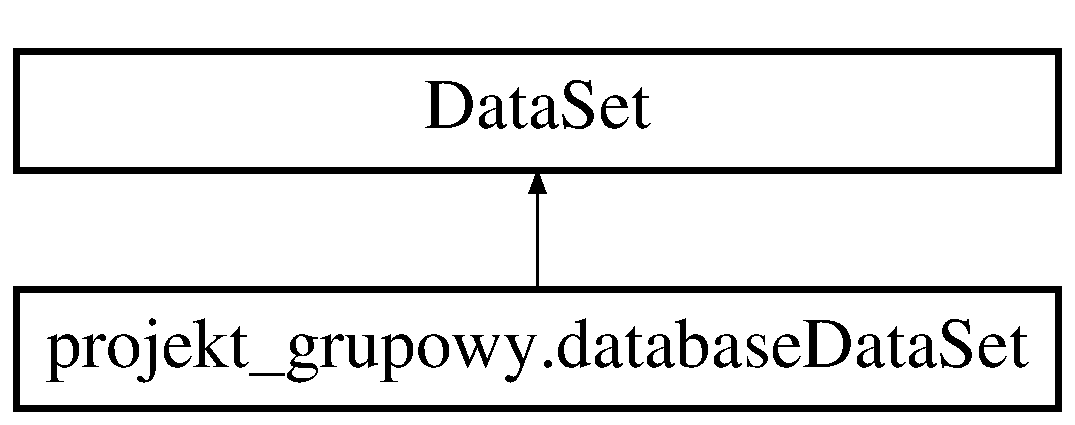
\includegraphics[height=2.000000cm]{classprojekt__grupowy_1_1database_data_set}
\end{center}
\end{figure}
\subsection*{Classes}
\begin{DoxyCompactItemize}
\item 
class \hyperlink{classprojekt__grupowy_1_1database_data_set_1_1_table_data_table}{Table\+Data\+Table}
\begin{DoxyCompactList}\small\item\em Represents the strongly named Data\+Table class. /summary$>$ \end{DoxyCompactList}\item 
class \hyperlink{classprojekt__grupowy_1_1database_data_set_1_1_table_row}{Table\+Row}
\begin{DoxyCompactList}\small\item\em Represents strongly named Data\+Row class. /summary$>$ \end{DoxyCompactList}\item 
class \hyperlink{classprojekt__grupowy_1_1database_data_set_1_1_table_row_change_event}{Table\+Row\+Change\+Event}
\begin{DoxyCompactList}\small\item\em Row event argument class /summary$>$ \end{DoxyCompactList}\end{DoxyCompactItemize}
\subsection*{Public Member Functions}
\begin{DoxyCompactItemize}
\item 
\mbox{\Hypertarget{classprojekt__grupowy_1_1database_data_set_aa22e2e2ac4597000732359cffed9cc7e}\label{classprojekt__grupowy_1_1database_data_set_aa22e2e2ac4597000732359cffed9cc7e}} 
override global\+::\+System.\+Data.\+Data\+Set {\bfseries Clone} ()
\item 
\mbox{\Hypertarget{classprojekt__grupowy_1_1database_data_set_aa2b7db7c2ea033ca442138077e1b1487}\label{classprojekt__grupowy_1_1database_data_set_aa2b7db7c2ea033ca442138077e1b1487}} 
delegate void {\bfseries Table\+Row\+Change\+Event\+Handler} (object sender, \hyperlink{classprojekt__grupowy_1_1database_data_set_1_1_table_row_change_event}{Table\+Row\+Change\+Event} e)
\end{DoxyCompactItemize}
\subsection*{Static Public Member Functions}
\begin{DoxyCompactItemize}
\item 
\mbox{\Hypertarget{classprojekt__grupowy_1_1database_data_set_a74fd701414f69b67e5d610bb7d8cc897}\label{classprojekt__grupowy_1_1database_data_set_a74fd701414f69b67e5d610bb7d8cc897}} 
static global\+::\+System.\+Xml.\+Schema.\+Xml\+Schema\+Complex\+Type {\bfseries Get\+Typed\+Data\+Set\+Schema} (global\+::\+System.\+Xml.\+Schema.\+Xml\+Schema\+Set xs)
\end{DoxyCompactItemize}
\subsection*{Protected Member Functions}
\begin{DoxyCompactItemize}
\item 
\mbox{\Hypertarget{classprojekt__grupowy_1_1database_data_set_ab74b74e969eca7357b0e7e329604751c}\label{classprojekt__grupowy_1_1database_data_set_ab74b74e969eca7357b0e7e329604751c}} 
{\bfseries database\+Data\+Set} (global\+::\+System.\+Runtime.\+Serialization.\+Serialization\+Info info, global\+::\+System.\+Runtime.\+Serialization.\+Streaming\+Context context)
\item 
\mbox{\Hypertarget{classprojekt__grupowy_1_1database_data_set_a3380af4a4b85afe3bea2af279a5d376e}\label{classprojekt__grupowy_1_1database_data_set_a3380af4a4b85afe3bea2af279a5d376e}} 
override void {\bfseries Initialize\+Derived\+Data\+Set} ()
\item 
\mbox{\Hypertarget{classprojekt__grupowy_1_1database_data_set_a053cf03aacbe58e75a0d6e2907bf6e57}\label{classprojekt__grupowy_1_1database_data_set_a053cf03aacbe58e75a0d6e2907bf6e57}} 
override bool {\bfseries Should\+Serialize\+Tables} ()
\item 
\mbox{\Hypertarget{classprojekt__grupowy_1_1database_data_set_ab57bb45894f4bd66c2e21dbcf547458e}\label{classprojekt__grupowy_1_1database_data_set_ab57bb45894f4bd66c2e21dbcf547458e}} 
override bool {\bfseries Should\+Serialize\+Relations} ()
\item 
\mbox{\Hypertarget{classprojekt__grupowy_1_1database_data_set_aa51deb6ae3ffc7beb179d57ee46c6712}\label{classprojekt__grupowy_1_1database_data_set_aa51deb6ae3ffc7beb179d57ee46c6712}} 
override void {\bfseries Read\+Xml\+Serializable} (global\+::\+System.\+Xml.\+Xml\+Reader reader)
\item 
\mbox{\Hypertarget{classprojekt__grupowy_1_1database_data_set_a246b77ef48cbef7fc969c08b36b3155f}\label{classprojekt__grupowy_1_1database_data_set_a246b77ef48cbef7fc969c08b36b3155f}} 
override global\+::\+System.\+Xml.\+Schema.\+Xml\+Schema {\bfseries Get\+Schema\+Serializable} ()
\end{DoxyCompactItemize}
\subsection*{Properties}
\begin{DoxyCompactItemize}
\item 
\mbox{\Hypertarget{classprojekt__grupowy_1_1database_data_set_a0a0d8615a12d80c1112395fe8c831243}\label{classprojekt__grupowy_1_1database_data_set_a0a0d8615a12d80c1112395fe8c831243}} 
\hyperlink{classprojekt__grupowy_1_1database_data_set_1_1_table_data_table}{Table\+Data\+Table} {\bfseries Table}\hspace{0.3cm}{\ttfamily  \mbox{[}get\mbox{]}}
\item 
\mbox{\Hypertarget{classprojekt__grupowy_1_1database_data_set_aca793fdd0b665ef1867d2abd09ee640a}\label{classprojekt__grupowy_1_1database_data_set_aca793fdd0b665ef1867d2abd09ee640a}} 
override global\+::\+System.\+Data.\+Schema\+Serialization\+Mode {\bfseries Schema\+Serialization\+Mode}\hspace{0.3cm}{\ttfamily  \mbox{[}get, set\mbox{]}}
\item 
\mbox{\Hypertarget{classprojekt__grupowy_1_1database_data_set_adff6a24f0cb8792b9deb60b3f49fad50}\label{classprojekt__grupowy_1_1database_data_set_adff6a24f0cb8792b9deb60b3f49fad50}} 
new global\+::\+System.\+Data.\+Data\+Table\+Collection {\bfseries Tables}\hspace{0.3cm}{\ttfamily  \mbox{[}get\mbox{]}}
\item 
\mbox{\Hypertarget{classprojekt__grupowy_1_1database_data_set_af0d5edeb9b8ed97111cbb0230f9a28fb}\label{classprojekt__grupowy_1_1database_data_set_af0d5edeb9b8ed97111cbb0230f9a28fb}} 
new global\+::\+System.\+Data.\+Data\+Relation\+Collection {\bfseries Relations}\hspace{0.3cm}{\ttfamily  \mbox{[}get\mbox{]}}
\end{DoxyCompactItemize}


\subsection{Detailed Description}
Represents a strongly typed in-\/memory cache of data. /summary$>$ 

The documentation for this class was generated from the following file\+:\begin{DoxyCompactItemize}
\item 
projekt\+\_\+grupowy/database\+Data\+Set.\+Designer.\+cs\end{DoxyCompactItemize}

\hypertarget{classprojekt__grupowy_1_1database_data_set1}{}\section{projekt\+\_\+grupowy.\+database\+Data\+Set1 Class Reference}
\label{classprojekt__grupowy_1_1database_data_set1}\index{projekt\+\_\+grupowy.\+database\+Data\+Set1@{projekt\+\_\+grupowy.\+database\+Data\+Set1}}


Represents a strongly typed in-\/memory cache of data. /summary$>$  


Inheritance diagram for projekt\+\_\+grupowy.\+database\+Data\+Set1\+:\begin{figure}[H]
\begin{center}
\leavevmode
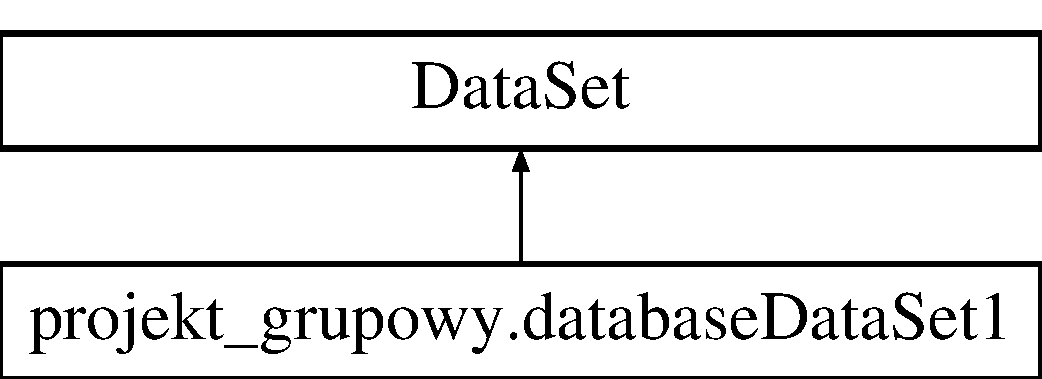
\includegraphics[height=2.000000cm]{classprojekt__grupowy_1_1database_data_set1}
\end{center}
\end{figure}
\subsection*{Classes}
\begin{DoxyCompactItemize}
\item 
class \hyperlink{classprojekt__grupowy_1_1database_data_set1_1_1_table_data_table}{Table\+Data\+Table}
\begin{DoxyCompactList}\small\item\em Represents the strongly named Data\+Table class. /summary$>$ \end{DoxyCompactList}\item 
class \hyperlink{classprojekt__grupowy_1_1database_data_set1_1_1_table_row}{Table\+Row}
\begin{DoxyCompactList}\small\item\em Represents strongly named Data\+Row class. /summary$>$ \end{DoxyCompactList}\item 
class \hyperlink{classprojekt__grupowy_1_1database_data_set1_1_1_table_row_change_event}{Table\+Row\+Change\+Event}
\begin{DoxyCompactList}\small\item\em Row event argument class /summary$>$ \end{DoxyCompactList}\end{DoxyCompactItemize}
\subsection*{Public Member Functions}
\begin{DoxyCompactItemize}
\item 
\mbox{\Hypertarget{classprojekt__grupowy_1_1database_data_set1_a18da6f77db71fac50fdeb88cd9847234}\label{classprojekt__grupowy_1_1database_data_set1_a18da6f77db71fac50fdeb88cd9847234}} 
override global\+::\+System.\+Data.\+Data\+Set {\bfseries Clone} ()
\item 
\mbox{\Hypertarget{classprojekt__grupowy_1_1database_data_set1_a10d76c3b643a3179cf094e6c4db20d66}\label{classprojekt__grupowy_1_1database_data_set1_a10d76c3b643a3179cf094e6c4db20d66}} 
delegate void {\bfseries Table\+Row\+Change\+Event\+Handler} (object sender, \hyperlink{classprojekt__grupowy_1_1database_data_set1_1_1_table_row_change_event}{Table\+Row\+Change\+Event} e)
\end{DoxyCompactItemize}
\subsection*{Static Public Member Functions}
\begin{DoxyCompactItemize}
\item 
\mbox{\Hypertarget{classprojekt__grupowy_1_1database_data_set1_abbc24ce53c73787e18955674655a00e9}\label{classprojekt__grupowy_1_1database_data_set1_abbc24ce53c73787e18955674655a00e9}} 
static global\+::\+System.\+Xml.\+Schema.\+Xml\+Schema\+Complex\+Type {\bfseries Get\+Typed\+Data\+Set\+Schema} (global\+::\+System.\+Xml.\+Schema.\+Xml\+Schema\+Set xs)
\end{DoxyCompactItemize}
\subsection*{Protected Member Functions}
\begin{DoxyCompactItemize}
\item 
\mbox{\Hypertarget{classprojekt__grupowy_1_1database_data_set1_a23b543373c1ac8f70dae82cb92a3cbbf}\label{classprojekt__grupowy_1_1database_data_set1_a23b543373c1ac8f70dae82cb92a3cbbf}} 
{\bfseries database\+Data\+Set1} (global\+::\+System.\+Runtime.\+Serialization.\+Serialization\+Info info, global\+::\+System.\+Runtime.\+Serialization.\+Streaming\+Context context)
\item 
\mbox{\Hypertarget{classprojekt__grupowy_1_1database_data_set1_abe6ee517fcdcf64c615aaf27c41b3765}\label{classprojekt__grupowy_1_1database_data_set1_abe6ee517fcdcf64c615aaf27c41b3765}} 
override void {\bfseries Initialize\+Derived\+Data\+Set} ()
\item 
\mbox{\Hypertarget{classprojekt__grupowy_1_1database_data_set1_acf83edfed0f908344cc99922e3862e73}\label{classprojekt__grupowy_1_1database_data_set1_acf83edfed0f908344cc99922e3862e73}} 
override bool {\bfseries Should\+Serialize\+Tables} ()
\item 
\mbox{\Hypertarget{classprojekt__grupowy_1_1database_data_set1_a1c99be96ad36bfb146f00c6a31410188}\label{classprojekt__grupowy_1_1database_data_set1_a1c99be96ad36bfb146f00c6a31410188}} 
override bool {\bfseries Should\+Serialize\+Relations} ()
\item 
\mbox{\Hypertarget{classprojekt__grupowy_1_1database_data_set1_aee2606d23b133be281612ca5f31b7505}\label{classprojekt__grupowy_1_1database_data_set1_aee2606d23b133be281612ca5f31b7505}} 
override void {\bfseries Read\+Xml\+Serializable} (global\+::\+System.\+Xml.\+Xml\+Reader reader)
\item 
\mbox{\Hypertarget{classprojekt__grupowy_1_1database_data_set1_a0a545d4d106212f1fd8a70a205d3ea72}\label{classprojekt__grupowy_1_1database_data_set1_a0a545d4d106212f1fd8a70a205d3ea72}} 
override global\+::\+System.\+Xml.\+Schema.\+Xml\+Schema {\bfseries Get\+Schema\+Serializable} ()
\end{DoxyCompactItemize}
\subsection*{Properties}
\begin{DoxyCompactItemize}
\item 
\mbox{\Hypertarget{classprojekt__grupowy_1_1database_data_set1_af278335abbd6be2ee023ce745714cacf}\label{classprojekt__grupowy_1_1database_data_set1_af278335abbd6be2ee023ce745714cacf}} 
\hyperlink{classprojekt__grupowy_1_1database_data_set1_1_1_table_data_table}{Table\+Data\+Table} {\bfseries Table}\hspace{0.3cm}{\ttfamily  \mbox{[}get\mbox{]}}
\item 
\mbox{\Hypertarget{classprojekt__grupowy_1_1database_data_set1_addafd3689f4e85dee9ce7c375a5d5a5e}\label{classprojekt__grupowy_1_1database_data_set1_addafd3689f4e85dee9ce7c375a5d5a5e}} 
override global\+::\+System.\+Data.\+Schema\+Serialization\+Mode {\bfseries Schema\+Serialization\+Mode}\hspace{0.3cm}{\ttfamily  \mbox{[}get, set\mbox{]}}
\item 
\mbox{\Hypertarget{classprojekt__grupowy_1_1database_data_set1_a48844d0d0248c84a68361dba6a3405c0}\label{classprojekt__grupowy_1_1database_data_set1_a48844d0d0248c84a68361dba6a3405c0}} 
new global\+::\+System.\+Data.\+Data\+Table\+Collection {\bfseries Tables}\hspace{0.3cm}{\ttfamily  \mbox{[}get\mbox{]}}
\item 
\mbox{\Hypertarget{classprojekt__grupowy_1_1database_data_set1_afba38adb4b0c9b2981f07f815c1ff029}\label{classprojekt__grupowy_1_1database_data_set1_afba38adb4b0c9b2981f07f815c1ff029}} 
new global\+::\+System.\+Data.\+Data\+Relation\+Collection {\bfseries Relations}\hspace{0.3cm}{\ttfamily  \mbox{[}get\mbox{]}}
\end{DoxyCompactItemize}


\subsection{Detailed Description}
Represents a strongly typed in-\/memory cache of data. /summary$>$ 

The documentation for this class was generated from the following file\+:\begin{DoxyCompactItemize}
\item 
projekt\+\_\+grupowy/database\+Data\+Set1.\+Designer.\+cs\end{DoxyCompactItemize}

\hypertarget{classprojekt__grupowy_1_1_form1}{}\section{projekt\+\_\+grupowy.\+Form1 Class Reference}
\label{classprojekt__grupowy_1_1_form1}\index{projekt\+\_\+grupowy.\+Form1@{projekt\+\_\+grupowy.\+Form1}}


The main form of the application.  


Inheritance diagram for projekt\+\_\+grupowy.\+Form1\+:\begin{figure}[H]
\begin{center}
\leavevmode
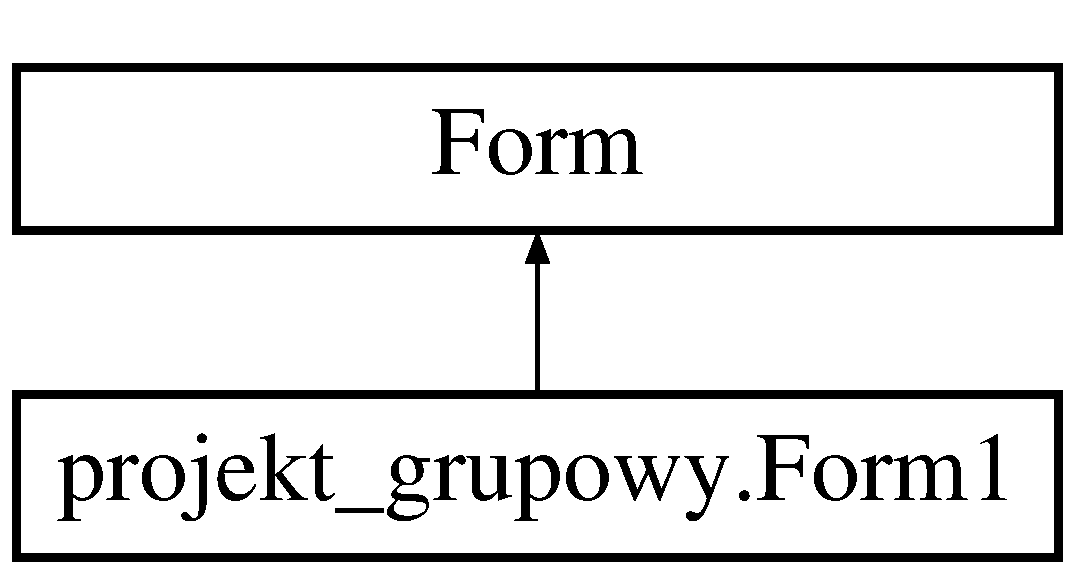
\includegraphics[height=2.000000cm]{classprojekt__grupowy_1_1_form1}
\end{center}
\end{figure}
\subsection*{Protected Member Functions}
\begin{DoxyCompactItemize}
\item 
override void \hyperlink{classprojekt__grupowy_1_1_form1_a87f3ce54094d8d3c419685438b224c9d}{Dispose} (bool disposing)
\begin{DoxyCompactList}\small\item\em Clean up any resources being used. \end{DoxyCompactList}\end{DoxyCompactItemize}


\subsection{Detailed Description}
The main form of the application. 



\subsection{Member Function Documentation}
\mbox{\Hypertarget{classprojekt__grupowy_1_1_form1_a87f3ce54094d8d3c419685438b224c9d}\label{classprojekt__grupowy_1_1_form1_a87f3ce54094d8d3c419685438b224c9d}} 
\index{projekt\+\_\+grupowy\+::\+Form1@{projekt\+\_\+grupowy\+::\+Form1}!Dispose@{Dispose}}
\index{Dispose@{Dispose}!projekt\+\_\+grupowy\+::\+Form1@{projekt\+\_\+grupowy\+::\+Form1}}
\subsubsection{\texorpdfstring{Dispose()}{Dispose()}}
{\footnotesize\ttfamily override void projekt\+\_\+grupowy.\+Form1.\+Dispose (\begin{DoxyParamCaption}\item[{bool}]{disposing }\end{DoxyParamCaption})\hspace{0.3cm}{\ttfamily [inline]}, {\ttfamily [protected]}}



Clean up any resources being used. 


\begin{DoxyParams}{Parameters}
{\em disposing} & true if managed resources should be disposed; otherwise, false.\\
\hline
\end{DoxyParams}


The documentation for this class was generated from the following files\+:\begin{DoxyCompactItemize}
\item 
projekt\+\_\+grupowy/Form1.\+cs\item 
projekt\+\_\+grupowy/Form1.\+Designer.\+cs\end{DoxyCompactItemize}

\hypertarget{classprojekt__grupowy_1_1database_data_set1_table_adapters_1_1_table_adapter_manager}{}\section{projekt\+\_\+grupowy.\+database\+Data\+Set1\+Table\+Adapters.\+Table\+Adapter\+Manager Class Reference}
\label{classprojekt__grupowy_1_1database_data_set1_table_adapters_1_1_table_adapter_manager}\index{projekt\+\_\+grupowy.\+database\+Data\+Set1\+Table\+Adapters.\+Table\+Adapter\+Manager@{projekt\+\_\+grupowy.\+database\+Data\+Set1\+Table\+Adapters.\+Table\+Adapter\+Manager}}


\hyperlink{classprojekt__grupowy_1_1database_data_set1_table_adapters_1_1_table_adapter_manager}{Table\+Adapter\+Manager} is used to coordinate Table\+Adapters in the dataset to enable Hierarchical Update scenarios /summary$>$  


Inheritance diagram for projekt\+\_\+grupowy.\+database\+Data\+Set1\+Table\+Adapters.\+Table\+Adapter\+Manager\+:\begin{figure}[H]
\begin{center}
\leavevmode
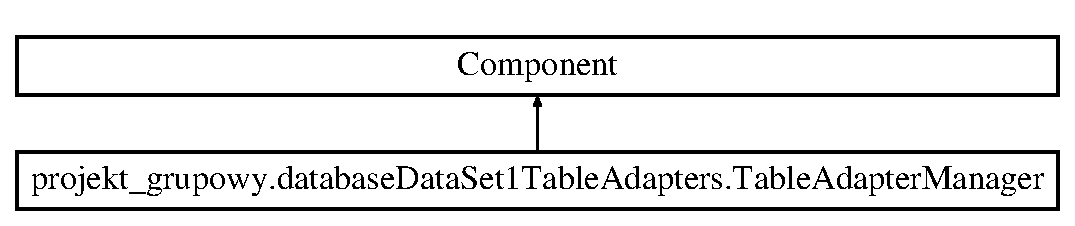
\includegraphics[height=2.000000cm]{classprojekt__grupowy_1_1database_data_set1_table_adapters_1_1_table_adapter_manager}
\end{center}
\end{figure}
\subsection*{Public Types}
\begin{DoxyCompactItemize}
\item 
\mbox{\Hypertarget{classprojekt__grupowy_1_1database_data_set1_table_adapters_1_1_table_adapter_manager_ad394b93344d1252bbb4268ccb8f786af}\label{classprojekt__grupowy_1_1database_data_set1_table_adapters_1_1_table_adapter_manager_ad394b93344d1252bbb4268ccb8f786af}} 
enum \hyperlink{classprojekt__grupowy_1_1database_data_set1_table_adapters_1_1_table_adapter_manager_ad394b93344d1252bbb4268ccb8f786af}{Update\+Order\+Option} \{ {\bfseries Insert\+Update\+Delete} = 0, 
{\bfseries Update\+Insert\+Delete} = 1
 \}\begin{DoxyCompactList}\small\item\em Update Order Option /summary$>$ \end{DoxyCompactList}
\end{DoxyCompactItemize}
\subsection*{Public Member Functions}
\begin{DoxyCompactItemize}
\item 
\mbox{\Hypertarget{classprojekt__grupowy_1_1database_data_set1_table_adapters_1_1_table_adapter_manager_a38426ebb65e6233c6fd1842095acb234}\label{classprojekt__grupowy_1_1database_data_set1_table_adapters_1_1_table_adapter_manager_a38426ebb65e6233c6fd1842095acb234}} 
virtual int \hyperlink{classprojekt__grupowy_1_1database_data_set1_table_adapters_1_1_table_adapter_manager_a38426ebb65e6233c6fd1842095acb234}{Update\+All} (\hyperlink{classprojekt__grupowy_1_1database_data_set1}{database\+Data\+Set1} data\+Set)
\begin{DoxyCompactList}\small\item\em Update all changes to the dataset. /summary$>$ \end{DoxyCompactList}\end{DoxyCompactItemize}
\subsection*{Protected Member Functions}
\begin{DoxyCompactItemize}
\item 
\mbox{\Hypertarget{classprojekt__grupowy_1_1database_data_set1_table_adapters_1_1_table_adapter_manager_a320d34e46e759b0a7f77e59ababa44d3}\label{classprojekt__grupowy_1_1database_data_set1_table_adapters_1_1_table_adapter_manager_a320d34e46e759b0a7f77e59ababa44d3}} 
virtual void {\bfseries Sort\+Self\+Reference\+Rows} (global\+::\+System.\+Data.\+Data\+Row\mbox{[}$\,$\mbox{]} rows, global\+::\+System.\+Data.\+Data\+Relation relation, bool child\+First)
\item 
\mbox{\Hypertarget{classprojekt__grupowy_1_1database_data_set1_table_adapters_1_1_table_adapter_manager_ac8b01e5580545e7014c9ad25a99f87a6}\label{classprojekt__grupowy_1_1database_data_set1_table_adapters_1_1_table_adapter_manager_ac8b01e5580545e7014c9ad25a99f87a6}} 
virtual bool {\bfseries Match\+Table\+Adapter\+Connection} (global\+::\+System.\+Data.\+I\+Db\+Connection input\+Connection)
\end{DoxyCompactItemize}
\subsection*{Properties}
\begin{DoxyCompactItemize}
\item 
\mbox{\Hypertarget{classprojekt__grupowy_1_1database_data_set1_table_adapters_1_1_table_adapter_manager_aa2369dfc1637ad014d736bc10adacc9c}\label{classprojekt__grupowy_1_1database_data_set1_table_adapters_1_1_table_adapter_manager_aa2369dfc1637ad014d736bc10adacc9c}} 
\hyperlink{classprojekt__grupowy_1_1database_data_set1_table_adapters_1_1_table_adapter_manager_ad394b93344d1252bbb4268ccb8f786af}{Update\+Order\+Option} {\bfseries Update\+Order}\hspace{0.3cm}{\ttfamily  \mbox{[}get, set\mbox{]}}
\item 
\mbox{\Hypertarget{classprojekt__grupowy_1_1database_data_set1_table_adapters_1_1_table_adapter_manager_ae2c71c45459a22745b27f2992746698e}\label{classprojekt__grupowy_1_1database_data_set1_table_adapters_1_1_table_adapter_manager_ae2c71c45459a22745b27f2992746698e}} 
\hyperlink{classprojekt__grupowy_1_1database_data_set1_table_adapters_1_1_table_table_adapter}{Table\+Table\+Adapter} {\bfseries Table\+Table\+Adapter}\hspace{0.3cm}{\ttfamily  \mbox{[}get, set\mbox{]}}
\item 
\mbox{\Hypertarget{classprojekt__grupowy_1_1database_data_set1_table_adapters_1_1_table_adapter_manager_a17ecbcbcf86cbd00a78f2e4b5a40525d}\label{classprojekt__grupowy_1_1database_data_set1_table_adapters_1_1_table_adapter_manager_a17ecbcbcf86cbd00a78f2e4b5a40525d}} 
bool {\bfseries Backup\+Data\+Set\+Before\+Update}\hspace{0.3cm}{\ttfamily  \mbox{[}get, set\mbox{]}}
\item 
\mbox{\Hypertarget{classprojekt__grupowy_1_1database_data_set1_table_adapters_1_1_table_adapter_manager_a76a181d57643bc6dccd00269d8179059}\label{classprojekt__grupowy_1_1database_data_set1_table_adapters_1_1_table_adapter_manager_a76a181d57643bc6dccd00269d8179059}} 
global\+::\+System.\+Data.\+I\+Db\+Connection {\bfseries Connection}\hspace{0.3cm}{\ttfamily  \mbox{[}get, set\mbox{]}}
\item 
\mbox{\Hypertarget{classprojekt__grupowy_1_1database_data_set1_table_adapters_1_1_table_adapter_manager_a7f9af27964a626ada1f841fc874af144}\label{classprojekt__grupowy_1_1database_data_set1_table_adapters_1_1_table_adapter_manager_a7f9af27964a626ada1f841fc874af144}} 
int {\bfseries Table\+Adapter\+Instance\+Count}\hspace{0.3cm}{\ttfamily  \mbox{[}get\mbox{]}}
\end{DoxyCompactItemize}


\subsection{Detailed Description}
\hyperlink{classprojekt__grupowy_1_1database_data_set1_table_adapters_1_1_table_adapter_manager}{Table\+Adapter\+Manager} is used to coordinate Table\+Adapters in the dataset to enable Hierarchical Update scenarios /summary$>$ 

The documentation for this class was generated from the following file\+:\begin{DoxyCompactItemize}
\item 
projekt\+\_\+grupowy/database\+Data\+Set1.\+Designer.\+cs\end{DoxyCompactItemize}

\hypertarget{classprojekt__grupowy_1_1database_data_set_table_adapters_1_1_table_adapter_manager}{}\section{projekt\+\_\+grupowy.\+database\+Data\+Set\+Table\+Adapters.\+Table\+Adapter\+Manager Class Reference}
\label{classprojekt__grupowy_1_1database_data_set_table_adapters_1_1_table_adapter_manager}\index{projekt\+\_\+grupowy.\+database\+Data\+Set\+Table\+Adapters.\+Table\+Adapter\+Manager@{projekt\+\_\+grupowy.\+database\+Data\+Set\+Table\+Adapters.\+Table\+Adapter\+Manager}}


\hyperlink{classprojekt__grupowy_1_1database_data_set_table_adapters_1_1_table_adapter_manager}{Table\+Adapter\+Manager} is used to coordinate Table\+Adapters in the dataset to enable Hierarchical Update scenarios /summary$>$  


Inheritance diagram for projekt\+\_\+grupowy.\+database\+Data\+Set\+Table\+Adapters.\+Table\+Adapter\+Manager\+:\begin{figure}[H]
\begin{center}
\leavevmode
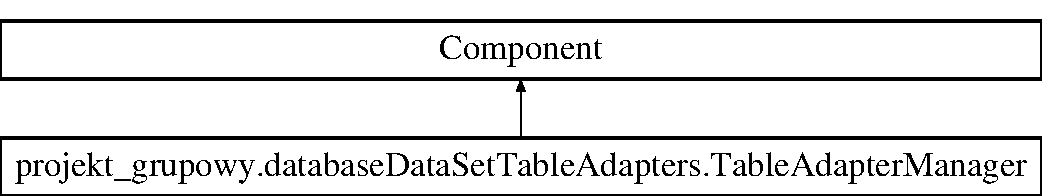
\includegraphics[height=2.000000cm]{classprojekt__grupowy_1_1database_data_set_table_adapters_1_1_table_adapter_manager}
\end{center}
\end{figure}
\subsection*{Public Types}
\begin{DoxyCompactItemize}
\item 
\mbox{\Hypertarget{classprojekt__grupowy_1_1database_data_set_table_adapters_1_1_table_adapter_manager_a28f63071f27298d15ff7cdcac275d946}\label{classprojekt__grupowy_1_1database_data_set_table_adapters_1_1_table_adapter_manager_a28f63071f27298d15ff7cdcac275d946}} 
enum \hyperlink{classprojekt__grupowy_1_1database_data_set_table_adapters_1_1_table_adapter_manager_a28f63071f27298d15ff7cdcac275d946}{Update\+Order\+Option} \{ {\bfseries Insert\+Update\+Delete} = 0, 
{\bfseries Update\+Insert\+Delete} = 1
 \}\begin{DoxyCompactList}\small\item\em Update Order Option /summary$>$ \end{DoxyCompactList}
\end{DoxyCompactItemize}
\subsection*{Public Member Functions}
\begin{DoxyCompactItemize}
\item 
\mbox{\Hypertarget{classprojekt__grupowy_1_1database_data_set_table_adapters_1_1_table_adapter_manager_aeffb3289e6b09ed0725b06ba7dae5b52}\label{classprojekt__grupowy_1_1database_data_set_table_adapters_1_1_table_adapter_manager_aeffb3289e6b09ed0725b06ba7dae5b52}} 
virtual int \hyperlink{classprojekt__grupowy_1_1database_data_set_table_adapters_1_1_table_adapter_manager_aeffb3289e6b09ed0725b06ba7dae5b52}{Update\+All} (\hyperlink{classprojekt__grupowy_1_1database_data_set}{database\+Data\+Set} data\+Set)
\begin{DoxyCompactList}\small\item\em Update all changes to the dataset. /summary$>$ \end{DoxyCompactList}\end{DoxyCompactItemize}
\subsection*{Protected Member Functions}
\begin{DoxyCompactItemize}
\item 
\mbox{\Hypertarget{classprojekt__grupowy_1_1database_data_set_table_adapters_1_1_table_adapter_manager_a9b1c956b09f3a4bb72df5b7487361383}\label{classprojekt__grupowy_1_1database_data_set_table_adapters_1_1_table_adapter_manager_a9b1c956b09f3a4bb72df5b7487361383}} 
virtual void {\bfseries Sort\+Self\+Reference\+Rows} (global\+::\+System.\+Data.\+Data\+Row\mbox{[}$\,$\mbox{]} rows, global\+::\+System.\+Data.\+Data\+Relation relation, bool child\+First)
\item 
\mbox{\Hypertarget{classprojekt__grupowy_1_1database_data_set_table_adapters_1_1_table_adapter_manager_a22bf35dba90267bdad45f13f88a71da8}\label{classprojekt__grupowy_1_1database_data_set_table_adapters_1_1_table_adapter_manager_a22bf35dba90267bdad45f13f88a71da8}} 
virtual bool {\bfseries Match\+Table\+Adapter\+Connection} (global\+::\+System.\+Data.\+I\+Db\+Connection input\+Connection)
\end{DoxyCompactItemize}
\subsection*{Properties}
\begin{DoxyCompactItemize}
\item 
\mbox{\Hypertarget{classprojekt__grupowy_1_1database_data_set_table_adapters_1_1_table_adapter_manager_ad6758d49bc505fa800f84cf129710a38}\label{classprojekt__grupowy_1_1database_data_set_table_adapters_1_1_table_adapter_manager_ad6758d49bc505fa800f84cf129710a38}} 
\hyperlink{classprojekt__grupowy_1_1database_data_set_table_adapters_1_1_table_adapter_manager_a28f63071f27298d15ff7cdcac275d946}{Update\+Order\+Option} {\bfseries Update\+Order}\hspace{0.3cm}{\ttfamily  \mbox{[}get, set\mbox{]}}
\item 
\mbox{\Hypertarget{classprojekt__grupowy_1_1database_data_set_table_adapters_1_1_table_adapter_manager_a1799c86b797bb2c87de60272743c9c2d}\label{classprojekt__grupowy_1_1database_data_set_table_adapters_1_1_table_adapter_manager_a1799c86b797bb2c87de60272743c9c2d}} 
\hyperlink{classprojekt__grupowy_1_1database_data_set_table_adapters_1_1_table_table_adapter}{Table\+Table\+Adapter} {\bfseries Table\+Table\+Adapter}\hspace{0.3cm}{\ttfamily  \mbox{[}get, set\mbox{]}}
\item 
\mbox{\Hypertarget{classprojekt__grupowy_1_1database_data_set_table_adapters_1_1_table_adapter_manager_a28e455cd91355446578dafbc850d4ad2}\label{classprojekt__grupowy_1_1database_data_set_table_adapters_1_1_table_adapter_manager_a28e455cd91355446578dafbc850d4ad2}} 
bool {\bfseries Backup\+Data\+Set\+Before\+Update}\hspace{0.3cm}{\ttfamily  \mbox{[}get, set\mbox{]}}
\item 
\mbox{\Hypertarget{classprojekt__grupowy_1_1database_data_set_table_adapters_1_1_table_adapter_manager_a85f5bfe3cbe25d5acc91a4929a815b12}\label{classprojekt__grupowy_1_1database_data_set_table_adapters_1_1_table_adapter_manager_a85f5bfe3cbe25d5acc91a4929a815b12}} 
global\+::\+System.\+Data.\+I\+Db\+Connection {\bfseries Connection}\hspace{0.3cm}{\ttfamily  \mbox{[}get, set\mbox{]}}
\item 
\mbox{\Hypertarget{classprojekt__grupowy_1_1database_data_set_table_adapters_1_1_table_adapter_manager_a4077699bf3ac701107fa0c4f3c24fbb4}\label{classprojekt__grupowy_1_1database_data_set_table_adapters_1_1_table_adapter_manager_a4077699bf3ac701107fa0c4f3c24fbb4}} 
int {\bfseries Table\+Adapter\+Instance\+Count}\hspace{0.3cm}{\ttfamily  \mbox{[}get\mbox{]}}
\end{DoxyCompactItemize}


\subsection{Detailed Description}
\hyperlink{classprojekt__grupowy_1_1database_data_set_table_adapters_1_1_table_adapter_manager}{Table\+Adapter\+Manager} is used to coordinate Table\+Adapters in the dataset to enable Hierarchical Update scenarios /summary$>$ 

The documentation for this class was generated from the following file\+:\begin{DoxyCompactItemize}
\item 
projekt\+\_\+grupowy/database\+Data\+Set.\+Designer.\+cs\end{DoxyCompactItemize}

\hypertarget{classprojekt__grupowy_1_1database_data_set_1_1_table_data_table}{}\section{projekt\+\_\+grupowy.\+database\+Data\+Set.\+Table\+Data\+Table Class Reference}
\label{classprojekt__grupowy_1_1database_data_set_1_1_table_data_table}\index{projekt\+\_\+grupowy.\+database\+Data\+Set.\+Table\+Data\+Table@{projekt\+\_\+grupowy.\+database\+Data\+Set.\+Table\+Data\+Table}}


Represents the strongly named Data\+Table class. /summary$>$  


Inheritance diagram for projekt\+\_\+grupowy.\+database\+Data\+Set.\+Table\+Data\+Table\+:\begin{figure}[H]
\begin{center}
\leavevmode
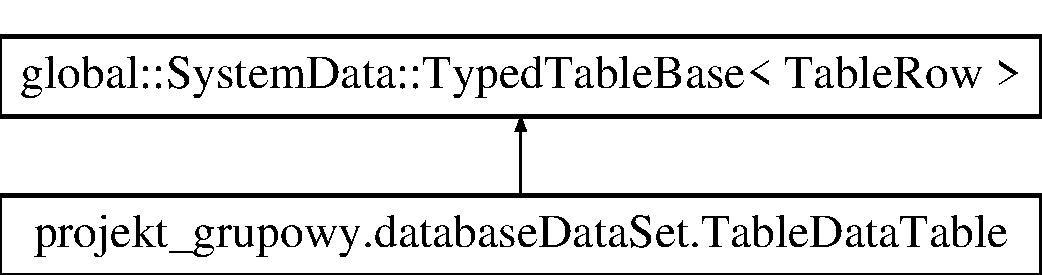
\includegraphics[height=2.000000cm]{classprojekt__grupowy_1_1database_data_set_1_1_table_data_table}
\end{center}
\end{figure}
\subsection*{Public Member Functions}
\begin{DoxyCompactItemize}
\item 
\mbox{\Hypertarget{classprojekt__grupowy_1_1database_data_set_1_1_table_data_table_af79a435292b98fa67d521c72dc754732}\label{classprojekt__grupowy_1_1database_data_set_1_1_table_data_table_af79a435292b98fa67d521c72dc754732}} 
void {\bfseries Add\+Table\+Row} (\hyperlink{classprojekt__grupowy_1_1database_data_set_1_1_table_row}{Table\+Row} row)
\item 
\mbox{\Hypertarget{classprojekt__grupowy_1_1database_data_set_1_1_table_data_table_ab62dde85c1f2c627f33ba437e23aff20}\label{classprojekt__grupowy_1_1database_data_set_1_1_table_data_table_ab62dde85c1f2c627f33ba437e23aff20}} 
\hyperlink{classprojekt__grupowy_1_1database_data_set_1_1_table_row}{Table\+Row} {\bfseries Add\+Table\+Row} (int Customer\+ID, string Name, string Surname, string Phone, string Brand, string Model)
\item 
\mbox{\Hypertarget{classprojekt__grupowy_1_1database_data_set_1_1_table_data_table_a84163598254bef73cb1dc52d24f9484c}\label{classprojekt__grupowy_1_1database_data_set_1_1_table_data_table_a84163598254bef73cb1dc52d24f9484c}} 
\hyperlink{classprojekt__grupowy_1_1database_data_set_1_1_table_row}{Table\+Row} {\bfseries Find\+By\+Customer\+ID} (int Customer\+ID)
\item 
\mbox{\Hypertarget{classprojekt__grupowy_1_1database_data_set_1_1_table_data_table_abd4bc44ad20793e5c391166804dd4e69}\label{classprojekt__grupowy_1_1database_data_set_1_1_table_data_table_abd4bc44ad20793e5c391166804dd4e69}} 
override global\+::\+System.\+Data.\+Data\+Table {\bfseries Clone} ()
\item 
\mbox{\Hypertarget{classprojekt__grupowy_1_1database_data_set_1_1_table_data_table_a6b1c8e429b95327f491a5e2dc4ab8e80}\label{classprojekt__grupowy_1_1database_data_set_1_1_table_data_table_a6b1c8e429b95327f491a5e2dc4ab8e80}} 
\hyperlink{classprojekt__grupowy_1_1database_data_set_1_1_table_row}{Table\+Row} {\bfseries New\+Table\+Row} ()
\item 
\mbox{\Hypertarget{classprojekt__grupowy_1_1database_data_set_1_1_table_data_table_aa57bf8c250286527bab038551fcffec8}\label{classprojekt__grupowy_1_1database_data_set_1_1_table_data_table_aa57bf8c250286527bab038551fcffec8}} 
void {\bfseries Remove\+Table\+Row} (\hyperlink{classprojekt__grupowy_1_1database_data_set_1_1_table_row}{Table\+Row} row)
\end{DoxyCompactItemize}
\subsection*{Static Public Member Functions}
\begin{DoxyCompactItemize}
\item 
\mbox{\Hypertarget{classprojekt__grupowy_1_1database_data_set_1_1_table_data_table_af35c27f1d4ea19bacabfafa0675115ff}\label{classprojekt__grupowy_1_1database_data_set_1_1_table_data_table_af35c27f1d4ea19bacabfafa0675115ff}} 
static global\+::\+System.\+Xml.\+Schema.\+Xml\+Schema\+Complex\+Type {\bfseries Get\+Typed\+Table\+Schema} (global\+::\+System.\+Xml.\+Schema.\+Xml\+Schema\+Set xs)
\end{DoxyCompactItemize}
\subsection*{Protected Member Functions}
\begin{DoxyCompactItemize}
\item 
\mbox{\Hypertarget{classprojekt__grupowy_1_1database_data_set_1_1_table_data_table_aa917c48c22b6e990d5c7a8290e6f182a}\label{classprojekt__grupowy_1_1database_data_set_1_1_table_data_table_aa917c48c22b6e990d5c7a8290e6f182a}} 
{\bfseries Table\+Data\+Table} (global\+::\+System.\+Runtime.\+Serialization.\+Serialization\+Info info, global\+::\+System.\+Runtime.\+Serialization.\+Streaming\+Context context)
\item 
\mbox{\Hypertarget{classprojekt__grupowy_1_1database_data_set_1_1_table_data_table_a83bb3a37743479e695dbf2be7b160b53}\label{classprojekt__grupowy_1_1database_data_set_1_1_table_data_table_a83bb3a37743479e695dbf2be7b160b53}} 
override global\+::\+System.\+Data.\+Data\+Table {\bfseries Create\+Instance} ()
\item 
\mbox{\Hypertarget{classprojekt__grupowy_1_1database_data_set_1_1_table_data_table_a1104d7433b495ddfc1c5bccd456f963e}\label{classprojekt__grupowy_1_1database_data_set_1_1_table_data_table_a1104d7433b495ddfc1c5bccd456f963e}} 
override global\+::\+System.\+Data.\+Data\+Row {\bfseries New\+Row\+From\+Builder} (global\+::\+System.\+Data.\+Data\+Row\+Builder builder)
\item 
\mbox{\Hypertarget{classprojekt__grupowy_1_1database_data_set_1_1_table_data_table_a3a5ca351995239d4e2dbdd1d44e28916}\label{classprojekt__grupowy_1_1database_data_set_1_1_table_data_table_a3a5ca351995239d4e2dbdd1d44e28916}} 
override global\+::\+System.\+Type {\bfseries Get\+Row\+Type} ()
\item 
\mbox{\Hypertarget{classprojekt__grupowy_1_1database_data_set_1_1_table_data_table_aed502d96df01aea981e69f60eebe8cec}\label{classprojekt__grupowy_1_1database_data_set_1_1_table_data_table_aed502d96df01aea981e69f60eebe8cec}} 
override void {\bfseries On\+Row\+Changed} (global\+::\+System.\+Data.\+Data\+Row\+Change\+Event\+Args e)
\item 
\mbox{\Hypertarget{classprojekt__grupowy_1_1database_data_set_1_1_table_data_table_a717bb54f7bcf5d92ac22306ac5448452}\label{classprojekt__grupowy_1_1database_data_set_1_1_table_data_table_a717bb54f7bcf5d92ac22306ac5448452}} 
override void {\bfseries On\+Row\+Changing} (global\+::\+System.\+Data.\+Data\+Row\+Change\+Event\+Args e)
\item 
\mbox{\Hypertarget{classprojekt__grupowy_1_1database_data_set_1_1_table_data_table_a94725a716824efcfe95c41cdfcf15afa}\label{classprojekt__grupowy_1_1database_data_set_1_1_table_data_table_a94725a716824efcfe95c41cdfcf15afa}} 
override void {\bfseries On\+Row\+Deleted} (global\+::\+System.\+Data.\+Data\+Row\+Change\+Event\+Args e)
\item 
\mbox{\Hypertarget{classprojekt__grupowy_1_1database_data_set_1_1_table_data_table_aed8df39c3436c3e3cd9969f5b40de6c1}\label{classprojekt__grupowy_1_1database_data_set_1_1_table_data_table_aed8df39c3436c3e3cd9969f5b40de6c1}} 
override void {\bfseries On\+Row\+Deleting} (global\+::\+System.\+Data.\+Data\+Row\+Change\+Event\+Args e)
\end{DoxyCompactItemize}
\subsection*{Properties}
\begin{DoxyCompactItemize}
\item 
\mbox{\Hypertarget{classprojekt__grupowy_1_1database_data_set_1_1_table_data_table_af3742a6a6c314590b9966b394dd22a03}\label{classprojekt__grupowy_1_1database_data_set_1_1_table_data_table_af3742a6a6c314590b9966b394dd22a03}} 
global\+::\+System.\+Data.\+Data\+Column {\bfseries Customer\+I\+D\+Column}\hspace{0.3cm}{\ttfamily  \mbox{[}get\mbox{]}}
\item 
\mbox{\Hypertarget{classprojekt__grupowy_1_1database_data_set_1_1_table_data_table_a399e570acfbbe5e00a37f1b4d37feaf8}\label{classprojekt__grupowy_1_1database_data_set_1_1_table_data_table_a399e570acfbbe5e00a37f1b4d37feaf8}} 
global\+::\+System.\+Data.\+Data\+Column {\bfseries Name\+Column}\hspace{0.3cm}{\ttfamily  \mbox{[}get\mbox{]}}
\item 
\mbox{\Hypertarget{classprojekt__grupowy_1_1database_data_set_1_1_table_data_table_a548e5d329427787bc13b9e0db2aa234e}\label{classprojekt__grupowy_1_1database_data_set_1_1_table_data_table_a548e5d329427787bc13b9e0db2aa234e}} 
global\+::\+System.\+Data.\+Data\+Column {\bfseries Surname\+Column}\hspace{0.3cm}{\ttfamily  \mbox{[}get\mbox{]}}
\item 
\mbox{\Hypertarget{classprojekt__grupowy_1_1database_data_set_1_1_table_data_table_a19ea528e0573e043008fee33f8855a67}\label{classprojekt__grupowy_1_1database_data_set_1_1_table_data_table_a19ea528e0573e043008fee33f8855a67}} 
global\+::\+System.\+Data.\+Data\+Column {\bfseries Phone\+Column}\hspace{0.3cm}{\ttfamily  \mbox{[}get\mbox{]}}
\item 
\mbox{\Hypertarget{classprojekt__grupowy_1_1database_data_set_1_1_table_data_table_a6337a45c488dfb857e967b6581f45d50}\label{classprojekt__grupowy_1_1database_data_set_1_1_table_data_table_a6337a45c488dfb857e967b6581f45d50}} 
global\+::\+System.\+Data.\+Data\+Column {\bfseries Brand\+Column}\hspace{0.3cm}{\ttfamily  \mbox{[}get\mbox{]}}
\item 
\mbox{\Hypertarget{classprojekt__grupowy_1_1database_data_set_1_1_table_data_table_a044bc90624b4cf26e7110fa96f7f896e}\label{classprojekt__grupowy_1_1database_data_set_1_1_table_data_table_a044bc90624b4cf26e7110fa96f7f896e}} 
global\+::\+System.\+Data.\+Data\+Column {\bfseries Model\+Column}\hspace{0.3cm}{\ttfamily  \mbox{[}get\mbox{]}}
\item 
\mbox{\Hypertarget{classprojekt__grupowy_1_1database_data_set_1_1_table_data_table_a460329b01a789832435bd9bd767c9726}\label{classprojekt__grupowy_1_1database_data_set_1_1_table_data_table_a460329b01a789832435bd9bd767c9726}} 
int {\bfseries Count}\hspace{0.3cm}{\ttfamily  \mbox{[}get\mbox{]}}
\item 
\mbox{\Hypertarget{classprojekt__grupowy_1_1database_data_set_1_1_table_data_table_a524e3d79fb8566d481eba6cc1872ad8f}\label{classprojekt__grupowy_1_1database_data_set_1_1_table_data_table_a524e3d79fb8566d481eba6cc1872ad8f}} 
\hyperlink{classprojekt__grupowy_1_1database_data_set_1_1_table_row}{Table\+Row} {\bfseries this\mbox{[}int index\mbox{]}}\hspace{0.3cm}{\ttfamily  \mbox{[}get\mbox{]}}
\end{DoxyCompactItemize}
\subsection*{Events}
\begin{DoxyCompactItemize}
\item 
\mbox{\Hypertarget{classprojekt__grupowy_1_1database_data_set_1_1_table_data_table_a2d8b09cf0c1630f4dc5c885713c81a34}\label{classprojekt__grupowy_1_1database_data_set_1_1_table_data_table_a2d8b09cf0c1630f4dc5c885713c81a34}} 
Table\+Row\+Change\+Event\+Handler {\bfseries Table\+Row\+Changing}
\item 
\mbox{\Hypertarget{classprojekt__grupowy_1_1database_data_set_1_1_table_data_table_aa4c852d00e655523289fba77beca7a94}\label{classprojekt__grupowy_1_1database_data_set_1_1_table_data_table_aa4c852d00e655523289fba77beca7a94}} 
Table\+Row\+Change\+Event\+Handler {\bfseries Table\+Row\+Changed}
\item 
\mbox{\Hypertarget{classprojekt__grupowy_1_1database_data_set_1_1_table_data_table_a2c7e6f1cc9ce77d8b01a3cffbb17ecc5}\label{classprojekt__grupowy_1_1database_data_set_1_1_table_data_table_a2c7e6f1cc9ce77d8b01a3cffbb17ecc5}} 
Table\+Row\+Change\+Event\+Handler {\bfseries Table\+Row\+Deleting}
\item 
\mbox{\Hypertarget{classprojekt__grupowy_1_1database_data_set_1_1_table_data_table_a9a1f955e4fd5f1bad61b44f5cd97a561}\label{classprojekt__grupowy_1_1database_data_set_1_1_table_data_table_a9a1f955e4fd5f1bad61b44f5cd97a561}} 
Table\+Row\+Change\+Event\+Handler {\bfseries Table\+Row\+Deleted}
\end{DoxyCompactItemize}


\subsection{Detailed Description}
Represents the strongly named Data\+Table class. /summary$>$ 

The documentation for this class was generated from the following file\+:\begin{DoxyCompactItemize}
\item 
projekt\+\_\+grupowy/database\+Data\+Set.\+Designer.\+cs\end{DoxyCompactItemize}

\hypertarget{classprojekt__grupowy_1_1database_data_set1_1_1_table_data_table}{}\section{projekt\+\_\+grupowy.\+database\+Data\+Set1.\+Table\+Data\+Table Class Reference}
\label{classprojekt__grupowy_1_1database_data_set1_1_1_table_data_table}\index{projekt\+\_\+grupowy.\+database\+Data\+Set1.\+Table\+Data\+Table@{projekt\+\_\+grupowy.\+database\+Data\+Set1.\+Table\+Data\+Table}}


Represents the strongly named Data\+Table class. /summary$>$  


Inheritance diagram for projekt\+\_\+grupowy.\+database\+Data\+Set1.\+Table\+Data\+Table\+:\begin{figure}[H]
\begin{center}
\leavevmode
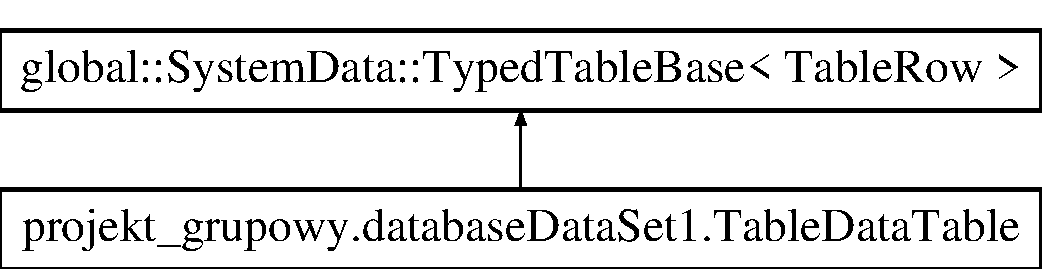
\includegraphics[height=2.000000cm]{classprojekt__grupowy_1_1database_data_set1_1_1_table_data_table}
\end{center}
\end{figure}
\subsection*{Public Member Functions}
\begin{DoxyCompactItemize}
\item 
\mbox{\Hypertarget{classprojekt__grupowy_1_1database_data_set1_1_1_table_data_table_a0e87c5d4fcafd15147cc3aad2a698ee0}\label{classprojekt__grupowy_1_1database_data_set1_1_1_table_data_table_a0e87c5d4fcafd15147cc3aad2a698ee0}} 
void {\bfseries Add\+Table\+Row} (\hyperlink{classprojekt__grupowy_1_1database_data_set1_1_1_table_row}{Table\+Row} row)
\item 
\mbox{\Hypertarget{classprojekt__grupowy_1_1database_data_set1_1_1_table_data_table_af8c7d84b49f2931cf4b7e0b358ba4873}\label{classprojekt__grupowy_1_1database_data_set1_1_1_table_data_table_af8c7d84b49f2931cf4b7e0b358ba4873}} 
\hyperlink{classprojekt__grupowy_1_1database_data_set1_1_1_table_row}{Table\+Row} {\bfseries Add\+Table\+Row} (int Customer\+ID, string Name, string Surname, string Phone, string Brand, string Model)
\item 
\mbox{\Hypertarget{classprojekt__grupowy_1_1database_data_set1_1_1_table_data_table_a128b88e58a07b07514cea04f3d91868f}\label{classprojekt__grupowy_1_1database_data_set1_1_1_table_data_table_a128b88e58a07b07514cea04f3d91868f}} 
\hyperlink{classprojekt__grupowy_1_1database_data_set1_1_1_table_row}{Table\+Row} {\bfseries Find\+By\+Customer\+ID} (int Customer\+ID)
\item 
\mbox{\Hypertarget{classprojekt__grupowy_1_1database_data_set1_1_1_table_data_table_aa01dfb0c435bd44ae82576752ff0f345}\label{classprojekt__grupowy_1_1database_data_set1_1_1_table_data_table_aa01dfb0c435bd44ae82576752ff0f345}} 
override global\+::\+System.\+Data.\+Data\+Table {\bfseries Clone} ()
\item 
\mbox{\Hypertarget{classprojekt__grupowy_1_1database_data_set1_1_1_table_data_table_a8632009bcffc0627a171fe37ada98295}\label{classprojekt__grupowy_1_1database_data_set1_1_1_table_data_table_a8632009bcffc0627a171fe37ada98295}} 
\hyperlink{classprojekt__grupowy_1_1database_data_set1_1_1_table_row}{Table\+Row} {\bfseries New\+Table\+Row} ()
\item 
\mbox{\Hypertarget{classprojekt__grupowy_1_1database_data_set1_1_1_table_data_table_a6ab3f3c4ad4b6d5809a88ef8f24eb29a}\label{classprojekt__grupowy_1_1database_data_set1_1_1_table_data_table_a6ab3f3c4ad4b6d5809a88ef8f24eb29a}} 
void {\bfseries Remove\+Table\+Row} (\hyperlink{classprojekt__grupowy_1_1database_data_set1_1_1_table_row}{Table\+Row} row)
\end{DoxyCompactItemize}
\subsection*{Static Public Member Functions}
\begin{DoxyCompactItemize}
\item 
\mbox{\Hypertarget{classprojekt__grupowy_1_1database_data_set1_1_1_table_data_table_ad1386f68765f8fe74aea3b3a83b4d6eb}\label{classprojekt__grupowy_1_1database_data_set1_1_1_table_data_table_ad1386f68765f8fe74aea3b3a83b4d6eb}} 
static global\+::\+System.\+Xml.\+Schema.\+Xml\+Schema\+Complex\+Type {\bfseries Get\+Typed\+Table\+Schema} (global\+::\+System.\+Xml.\+Schema.\+Xml\+Schema\+Set xs)
\end{DoxyCompactItemize}
\subsection*{Protected Member Functions}
\begin{DoxyCompactItemize}
\item 
\mbox{\Hypertarget{classprojekt__grupowy_1_1database_data_set1_1_1_table_data_table_ac0995da5cb120357cb3af240467de6f1}\label{classprojekt__grupowy_1_1database_data_set1_1_1_table_data_table_ac0995da5cb120357cb3af240467de6f1}} 
{\bfseries Table\+Data\+Table} (global\+::\+System.\+Runtime.\+Serialization.\+Serialization\+Info info, global\+::\+System.\+Runtime.\+Serialization.\+Streaming\+Context context)
\item 
\mbox{\Hypertarget{classprojekt__grupowy_1_1database_data_set1_1_1_table_data_table_a4ffd6a51c1c4c0a27c8a012bc6db94a1}\label{classprojekt__grupowy_1_1database_data_set1_1_1_table_data_table_a4ffd6a51c1c4c0a27c8a012bc6db94a1}} 
override global\+::\+System.\+Data.\+Data\+Table {\bfseries Create\+Instance} ()
\item 
\mbox{\Hypertarget{classprojekt__grupowy_1_1database_data_set1_1_1_table_data_table_a61b91c7eafce70ab6709152f96f77386}\label{classprojekt__grupowy_1_1database_data_set1_1_1_table_data_table_a61b91c7eafce70ab6709152f96f77386}} 
override global\+::\+System.\+Data.\+Data\+Row {\bfseries New\+Row\+From\+Builder} (global\+::\+System.\+Data.\+Data\+Row\+Builder builder)
\item 
\mbox{\Hypertarget{classprojekt__grupowy_1_1database_data_set1_1_1_table_data_table_a3cbf6074bb047e88fa88f6568589eb32}\label{classprojekt__grupowy_1_1database_data_set1_1_1_table_data_table_a3cbf6074bb047e88fa88f6568589eb32}} 
override global\+::\+System.\+Type {\bfseries Get\+Row\+Type} ()
\item 
\mbox{\Hypertarget{classprojekt__grupowy_1_1database_data_set1_1_1_table_data_table_aa4281e17997c8b233a81a69fc9261c2c}\label{classprojekt__grupowy_1_1database_data_set1_1_1_table_data_table_aa4281e17997c8b233a81a69fc9261c2c}} 
override void {\bfseries On\+Row\+Changed} (global\+::\+System.\+Data.\+Data\+Row\+Change\+Event\+Args e)
\item 
\mbox{\Hypertarget{classprojekt__grupowy_1_1database_data_set1_1_1_table_data_table_a02e53176dc2fcbb4a0bf31f99e1a4309}\label{classprojekt__grupowy_1_1database_data_set1_1_1_table_data_table_a02e53176dc2fcbb4a0bf31f99e1a4309}} 
override void {\bfseries On\+Row\+Changing} (global\+::\+System.\+Data.\+Data\+Row\+Change\+Event\+Args e)
\item 
\mbox{\Hypertarget{classprojekt__grupowy_1_1database_data_set1_1_1_table_data_table_abbe092066f472ddabc2eb44f3ffd666b}\label{classprojekt__grupowy_1_1database_data_set1_1_1_table_data_table_abbe092066f472ddabc2eb44f3ffd666b}} 
override void {\bfseries On\+Row\+Deleted} (global\+::\+System.\+Data.\+Data\+Row\+Change\+Event\+Args e)
\item 
\mbox{\Hypertarget{classprojekt__grupowy_1_1database_data_set1_1_1_table_data_table_a904da21b62e463d68564943e084165bb}\label{classprojekt__grupowy_1_1database_data_set1_1_1_table_data_table_a904da21b62e463d68564943e084165bb}} 
override void {\bfseries On\+Row\+Deleting} (global\+::\+System.\+Data.\+Data\+Row\+Change\+Event\+Args e)
\end{DoxyCompactItemize}
\subsection*{Properties}
\begin{DoxyCompactItemize}
\item 
\mbox{\Hypertarget{classprojekt__grupowy_1_1database_data_set1_1_1_table_data_table_a45085a95ab7115ffdc49eee2f8793344}\label{classprojekt__grupowy_1_1database_data_set1_1_1_table_data_table_a45085a95ab7115ffdc49eee2f8793344}} 
global\+::\+System.\+Data.\+Data\+Column {\bfseries Customer\+I\+D\+Column}\hspace{0.3cm}{\ttfamily  \mbox{[}get\mbox{]}}
\item 
\mbox{\Hypertarget{classprojekt__grupowy_1_1database_data_set1_1_1_table_data_table_a5af65a83a2c2e5c3770bdbb1faee100c}\label{classprojekt__grupowy_1_1database_data_set1_1_1_table_data_table_a5af65a83a2c2e5c3770bdbb1faee100c}} 
global\+::\+System.\+Data.\+Data\+Column {\bfseries Name\+Column}\hspace{0.3cm}{\ttfamily  \mbox{[}get\mbox{]}}
\item 
\mbox{\Hypertarget{classprojekt__grupowy_1_1database_data_set1_1_1_table_data_table_a5a0399d18cd860bb90acf30fee080e5a}\label{classprojekt__grupowy_1_1database_data_set1_1_1_table_data_table_a5a0399d18cd860bb90acf30fee080e5a}} 
global\+::\+System.\+Data.\+Data\+Column {\bfseries Surname\+Column}\hspace{0.3cm}{\ttfamily  \mbox{[}get\mbox{]}}
\item 
\mbox{\Hypertarget{classprojekt__grupowy_1_1database_data_set1_1_1_table_data_table_aa7029cdc183f4a95cc1a8a3967e1cf5b}\label{classprojekt__grupowy_1_1database_data_set1_1_1_table_data_table_aa7029cdc183f4a95cc1a8a3967e1cf5b}} 
global\+::\+System.\+Data.\+Data\+Column {\bfseries Phone\+Column}\hspace{0.3cm}{\ttfamily  \mbox{[}get\mbox{]}}
\item 
\mbox{\Hypertarget{classprojekt__grupowy_1_1database_data_set1_1_1_table_data_table_a99d1062ee06755a610e8200cf42c92be}\label{classprojekt__grupowy_1_1database_data_set1_1_1_table_data_table_a99d1062ee06755a610e8200cf42c92be}} 
global\+::\+System.\+Data.\+Data\+Column {\bfseries Brand\+Column}\hspace{0.3cm}{\ttfamily  \mbox{[}get\mbox{]}}
\item 
\mbox{\Hypertarget{classprojekt__grupowy_1_1database_data_set1_1_1_table_data_table_a0e91ac674afd8e0e270e56094c3c2528}\label{classprojekt__grupowy_1_1database_data_set1_1_1_table_data_table_a0e91ac674afd8e0e270e56094c3c2528}} 
global\+::\+System.\+Data.\+Data\+Column {\bfseries Model\+Column}\hspace{0.3cm}{\ttfamily  \mbox{[}get\mbox{]}}
\item 
\mbox{\Hypertarget{classprojekt__grupowy_1_1database_data_set1_1_1_table_data_table_a3b3df0db393872b770f569d6165a54f6}\label{classprojekt__grupowy_1_1database_data_set1_1_1_table_data_table_a3b3df0db393872b770f569d6165a54f6}} 
int {\bfseries Count}\hspace{0.3cm}{\ttfamily  \mbox{[}get\mbox{]}}
\item 
\mbox{\Hypertarget{classprojekt__grupowy_1_1database_data_set1_1_1_table_data_table_abff84451373570e4edeb04360c8940c5}\label{classprojekt__grupowy_1_1database_data_set1_1_1_table_data_table_abff84451373570e4edeb04360c8940c5}} 
\hyperlink{classprojekt__grupowy_1_1database_data_set1_1_1_table_row}{Table\+Row} {\bfseries this\mbox{[}int index\mbox{]}}\hspace{0.3cm}{\ttfamily  \mbox{[}get\mbox{]}}
\end{DoxyCompactItemize}
\subsection*{Events}
\begin{DoxyCompactItemize}
\item 
\mbox{\Hypertarget{classprojekt__grupowy_1_1database_data_set1_1_1_table_data_table_a95b49a5f2754ed9d77c5973161a3510b}\label{classprojekt__grupowy_1_1database_data_set1_1_1_table_data_table_a95b49a5f2754ed9d77c5973161a3510b}} 
Table\+Row\+Change\+Event\+Handler {\bfseries Table\+Row\+Changing}
\item 
\mbox{\Hypertarget{classprojekt__grupowy_1_1database_data_set1_1_1_table_data_table_a40baae85167732e87dbdf160f720c7e9}\label{classprojekt__grupowy_1_1database_data_set1_1_1_table_data_table_a40baae85167732e87dbdf160f720c7e9}} 
Table\+Row\+Change\+Event\+Handler {\bfseries Table\+Row\+Changed}
\item 
\mbox{\Hypertarget{classprojekt__grupowy_1_1database_data_set1_1_1_table_data_table_ae9f5743fb89ef52cefedcc9b89288ef0}\label{classprojekt__grupowy_1_1database_data_set1_1_1_table_data_table_ae9f5743fb89ef52cefedcc9b89288ef0}} 
Table\+Row\+Change\+Event\+Handler {\bfseries Table\+Row\+Deleting}
\item 
\mbox{\Hypertarget{classprojekt__grupowy_1_1database_data_set1_1_1_table_data_table_a769205cec3478233cddcf78dfee38fc2}\label{classprojekt__grupowy_1_1database_data_set1_1_1_table_data_table_a769205cec3478233cddcf78dfee38fc2}} 
Table\+Row\+Change\+Event\+Handler {\bfseries Table\+Row\+Deleted}
\end{DoxyCompactItemize}


\subsection{Detailed Description}
Represents the strongly named Data\+Table class. /summary$>$ 

The documentation for this class was generated from the following file\+:\begin{DoxyCompactItemize}
\item 
projekt\+\_\+grupowy/database\+Data\+Set1.\+Designer.\+cs\end{DoxyCompactItemize}

\hypertarget{classprojekt__grupowy_1_1database_data_set1_1_1_table_row}{}\section{projekt\+\_\+grupowy.\+database\+Data\+Set1.\+Table\+Row Class Reference}
\label{classprojekt__grupowy_1_1database_data_set1_1_1_table_row}\index{projekt\+\_\+grupowy.\+database\+Data\+Set1.\+Table\+Row@{projekt\+\_\+grupowy.\+database\+Data\+Set1.\+Table\+Row}}


Represents strongly named Data\+Row class. /summary$>$  


Inheritance diagram for projekt\+\_\+grupowy.\+database\+Data\+Set1.\+Table\+Row\+:\begin{figure}[H]
\begin{center}
\leavevmode
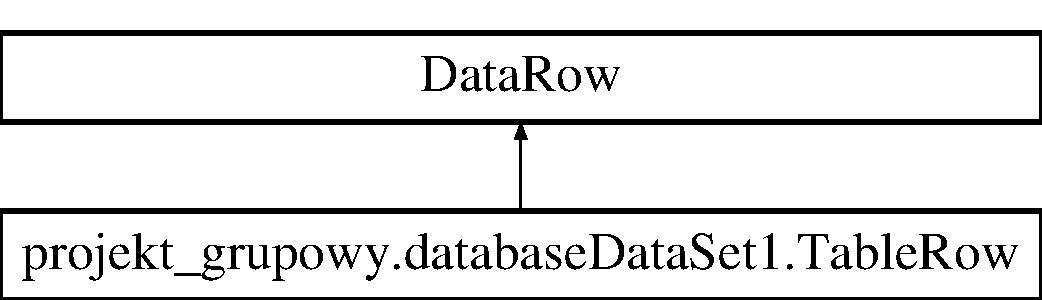
\includegraphics[height=2.000000cm]{classprojekt__grupowy_1_1database_data_set1_1_1_table_row}
\end{center}
\end{figure}
\subsection*{Public Member Functions}
\begin{DoxyCompactItemize}
\item 
\mbox{\Hypertarget{classprojekt__grupowy_1_1database_data_set1_1_1_table_row_a4cef8b8490bd4de00ba553fd9c08b005}\label{classprojekt__grupowy_1_1database_data_set1_1_1_table_row_a4cef8b8490bd4de00ba553fd9c08b005}} 
bool {\bfseries Is\+Name\+Null} ()
\item 
\mbox{\Hypertarget{classprojekt__grupowy_1_1database_data_set1_1_1_table_row_a7ae581270662300532e7d46c9b5d1f10}\label{classprojekt__grupowy_1_1database_data_set1_1_1_table_row_a7ae581270662300532e7d46c9b5d1f10}} 
void {\bfseries Set\+Name\+Null} ()
\item 
\mbox{\Hypertarget{classprojekt__grupowy_1_1database_data_set1_1_1_table_row_a227f1aa540cf8d3fb0b97f1247723bc7}\label{classprojekt__grupowy_1_1database_data_set1_1_1_table_row_a227f1aa540cf8d3fb0b97f1247723bc7}} 
bool {\bfseries Is\+Surname\+Null} ()
\item 
\mbox{\Hypertarget{classprojekt__grupowy_1_1database_data_set1_1_1_table_row_a516542cc353ab176923a10336321d311}\label{classprojekt__grupowy_1_1database_data_set1_1_1_table_row_a516542cc353ab176923a10336321d311}} 
void {\bfseries Set\+Surname\+Null} ()
\item 
\mbox{\Hypertarget{classprojekt__grupowy_1_1database_data_set1_1_1_table_row_a2219aa70ec7c4a1d6124f898489f783f}\label{classprojekt__grupowy_1_1database_data_set1_1_1_table_row_a2219aa70ec7c4a1d6124f898489f783f}} 
bool {\bfseries Is\+Phone\+Null} ()
\item 
\mbox{\Hypertarget{classprojekt__grupowy_1_1database_data_set1_1_1_table_row_aa22906e64679e825aec9878dfb7e6306}\label{classprojekt__grupowy_1_1database_data_set1_1_1_table_row_aa22906e64679e825aec9878dfb7e6306}} 
void {\bfseries Set\+Phone\+Null} ()
\item 
\mbox{\Hypertarget{classprojekt__grupowy_1_1database_data_set1_1_1_table_row_a9a574f0228501499bcd7e6eefb2d9ac7}\label{classprojekt__grupowy_1_1database_data_set1_1_1_table_row_a9a574f0228501499bcd7e6eefb2d9ac7}} 
bool {\bfseries Is\+Brand\+Null} ()
\item 
\mbox{\Hypertarget{classprojekt__grupowy_1_1database_data_set1_1_1_table_row_afcfcbfa83e95202594cc04550a7b41ec}\label{classprojekt__grupowy_1_1database_data_set1_1_1_table_row_afcfcbfa83e95202594cc04550a7b41ec}} 
void {\bfseries Set\+Brand\+Null} ()
\item 
\mbox{\Hypertarget{classprojekt__grupowy_1_1database_data_set1_1_1_table_row_a212eb0864fb67344273954eae207e761}\label{classprojekt__grupowy_1_1database_data_set1_1_1_table_row_a212eb0864fb67344273954eae207e761}} 
bool {\bfseries Is\+Model\+Null} ()
\item 
\mbox{\Hypertarget{classprojekt__grupowy_1_1database_data_set1_1_1_table_row_a617f99398aaab810102a5bc51c45d9b5}\label{classprojekt__grupowy_1_1database_data_set1_1_1_table_row_a617f99398aaab810102a5bc51c45d9b5}} 
void {\bfseries Set\+Model\+Null} ()
\end{DoxyCompactItemize}
\subsection*{Properties}
\begin{DoxyCompactItemize}
\item 
\mbox{\Hypertarget{classprojekt__grupowy_1_1database_data_set1_1_1_table_row_a8d784095200fa90809d00060a9dd55db}\label{classprojekt__grupowy_1_1database_data_set1_1_1_table_row_a8d784095200fa90809d00060a9dd55db}} 
int {\bfseries Customer\+ID}\hspace{0.3cm}{\ttfamily  \mbox{[}get, set\mbox{]}}
\item 
\mbox{\Hypertarget{classprojekt__grupowy_1_1database_data_set1_1_1_table_row_a31264e7ec5685a784465f6f85889fb73}\label{classprojekt__grupowy_1_1database_data_set1_1_1_table_row_a31264e7ec5685a784465f6f85889fb73}} 
string {\bfseries Name}\hspace{0.3cm}{\ttfamily  \mbox{[}get, set\mbox{]}}
\item 
\mbox{\Hypertarget{classprojekt__grupowy_1_1database_data_set1_1_1_table_row_afec939c8383599a8e332dd1987a94375}\label{classprojekt__grupowy_1_1database_data_set1_1_1_table_row_afec939c8383599a8e332dd1987a94375}} 
string {\bfseries Surname}\hspace{0.3cm}{\ttfamily  \mbox{[}get, set\mbox{]}}
\item 
\mbox{\Hypertarget{classprojekt__grupowy_1_1database_data_set1_1_1_table_row_ab6639fb215f263ee8dd928b63667df1b}\label{classprojekt__grupowy_1_1database_data_set1_1_1_table_row_ab6639fb215f263ee8dd928b63667df1b}} 
string {\bfseries Phone}\hspace{0.3cm}{\ttfamily  \mbox{[}get, set\mbox{]}}
\item 
\mbox{\Hypertarget{classprojekt__grupowy_1_1database_data_set1_1_1_table_row_a922cebc6492c4fc678972fd2759f5021}\label{classprojekt__grupowy_1_1database_data_set1_1_1_table_row_a922cebc6492c4fc678972fd2759f5021}} 
string {\bfseries Brand}\hspace{0.3cm}{\ttfamily  \mbox{[}get, set\mbox{]}}
\item 
\mbox{\Hypertarget{classprojekt__grupowy_1_1database_data_set1_1_1_table_row_aaa773bfb7b5ea928e76639ab320a5ce2}\label{classprojekt__grupowy_1_1database_data_set1_1_1_table_row_aaa773bfb7b5ea928e76639ab320a5ce2}} 
string {\bfseries Model}\hspace{0.3cm}{\ttfamily  \mbox{[}get, set\mbox{]}}
\end{DoxyCompactItemize}


\subsection{Detailed Description}
Represents strongly named Data\+Row class. /summary$>$ 

The documentation for this class was generated from the following file\+:\begin{DoxyCompactItemize}
\item 
projekt\+\_\+grupowy/database\+Data\+Set1.\+Designer.\+cs\end{DoxyCompactItemize}

\hypertarget{classprojekt__grupowy_1_1database_data_set_1_1_table_row}{}\section{projekt\+\_\+grupowy.\+database\+Data\+Set.\+Table\+Row Class Reference}
\label{classprojekt__grupowy_1_1database_data_set_1_1_table_row}\index{projekt\+\_\+grupowy.\+database\+Data\+Set.\+Table\+Row@{projekt\+\_\+grupowy.\+database\+Data\+Set.\+Table\+Row}}


Represents strongly named Data\+Row class. /summary$>$  


Inheritance diagram for projekt\+\_\+grupowy.\+database\+Data\+Set.\+Table\+Row\+:\begin{figure}[H]
\begin{center}
\leavevmode
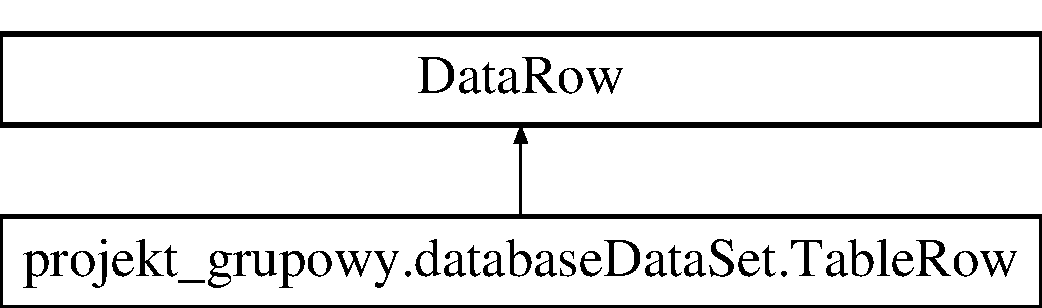
\includegraphics[height=2.000000cm]{classprojekt__grupowy_1_1database_data_set_1_1_table_row}
\end{center}
\end{figure}
\subsection*{Public Member Functions}
\begin{DoxyCompactItemize}
\item 
\mbox{\Hypertarget{classprojekt__grupowy_1_1database_data_set_1_1_table_row_abb9dae935364f9b269cacca2600c2809}\label{classprojekt__grupowy_1_1database_data_set_1_1_table_row_abb9dae935364f9b269cacca2600c2809}} 
bool {\bfseries Is\+Name\+Null} ()
\item 
\mbox{\Hypertarget{classprojekt__grupowy_1_1database_data_set_1_1_table_row_ac3fbcd96103ff22f3a44b7aa16949076}\label{classprojekt__grupowy_1_1database_data_set_1_1_table_row_ac3fbcd96103ff22f3a44b7aa16949076}} 
void {\bfseries Set\+Name\+Null} ()
\item 
\mbox{\Hypertarget{classprojekt__grupowy_1_1database_data_set_1_1_table_row_af99e51c6600364b3d94860b8b15c385d}\label{classprojekt__grupowy_1_1database_data_set_1_1_table_row_af99e51c6600364b3d94860b8b15c385d}} 
bool {\bfseries Is\+Surname\+Null} ()
\item 
\mbox{\Hypertarget{classprojekt__grupowy_1_1database_data_set_1_1_table_row_ae499e572c5ba58b3dcb873aef73f2e13}\label{classprojekt__grupowy_1_1database_data_set_1_1_table_row_ae499e572c5ba58b3dcb873aef73f2e13}} 
void {\bfseries Set\+Surname\+Null} ()
\item 
\mbox{\Hypertarget{classprojekt__grupowy_1_1database_data_set_1_1_table_row_ad533e31c2c8b0261e7997eb6e15dd929}\label{classprojekt__grupowy_1_1database_data_set_1_1_table_row_ad533e31c2c8b0261e7997eb6e15dd929}} 
bool {\bfseries Is\+Phone\+Null} ()
\item 
\mbox{\Hypertarget{classprojekt__grupowy_1_1database_data_set_1_1_table_row_a9bb22b0efbf7e9ae9760aef241fc6af7}\label{classprojekt__grupowy_1_1database_data_set_1_1_table_row_a9bb22b0efbf7e9ae9760aef241fc6af7}} 
void {\bfseries Set\+Phone\+Null} ()
\item 
\mbox{\Hypertarget{classprojekt__grupowy_1_1database_data_set_1_1_table_row_a26ff39d444442514dc7e1f771b8fac87}\label{classprojekt__grupowy_1_1database_data_set_1_1_table_row_a26ff39d444442514dc7e1f771b8fac87}} 
bool {\bfseries Is\+Brand\+Null} ()
\item 
\mbox{\Hypertarget{classprojekt__grupowy_1_1database_data_set_1_1_table_row_a9330170081a8a87b0af629f79193cc46}\label{classprojekt__grupowy_1_1database_data_set_1_1_table_row_a9330170081a8a87b0af629f79193cc46}} 
void {\bfseries Set\+Brand\+Null} ()
\item 
\mbox{\Hypertarget{classprojekt__grupowy_1_1database_data_set_1_1_table_row_a6249607cf7f5f31cad8e9b9e7c526daf}\label{classprojekt__grupowy_1_1database_data_set_1_1_table_row_a6249607cf7f5f31cad8e9b9e7c526daf}} 
bool {\bfseries Is\+Model\+Null} ()
\item 
\mbox{\Hypertarget{classprojekt__grupowy_1_1database_data_set_1_1_table_row_a415c333b4db34fdd736a1a38e5016fb6}\label{classprojekt__grupowy_1_1database_data_set_1_1_table_row_a415c333b4db34fdd736a1a38e5016fb6}} 
void {\bfseries Set\+Model\+Null} ()
\end{DoxyCompactItemize}
\subsection*{Properties}
\begin{DoxyCompactItemize}
\item 
\mbox{\Hypertarget{classprojekt__grupowy_1_1database_data_set_1_1_table_row_acca10b3fee85160e8b31dd4831b2e4aa}\label{classprojekt__grupowy_1_1database_data_set_1_1_table_row_acca10b3fee85160e8b31dd4831b2e4aa}} 
int {\bfseries Customer\+ID}\hspace{0.3cm}{\ttfamily  \mbox{[}get, set\mbox{]}}
\item 
\mbox{\Hypertarget{classprojekt__grupowy_1_1database_data_set_1_1_table_row_a580e3324a8bf4643dd118da776260521}\label{classprojekt__grupowy_1_1database_data_set_1_1_table_row_a580e3324a8bf4643dd118da776260521}} 
string {\bfseries Name}\hspace{0.3cm}{\ttfamily  \mbox{[}get, set\mbox{]}}
\item 
\mbox{\Hypertarget{classprojekt__grupowy_1_1database_data_set_1_1_table_row_a8e5f9e1d022e0c91568c8bdbd68de382}\label{classprojekt__grupowy_1_1database_data_set_1_1_table_row_a8e5f9e1d022e0c91568c8bdbd68de382}} 
string {\bfseries Surname}\hspace{0.3cm}{\ttfamily  \mbox{[}get, set\mbox{]}}
\item 
\mbox{\Hypertarget{classprojekt__grupowy_1_1database_data_set_1_1_table_row_af2371ee7c8b41e1c4b8caa0132e5dcb1}\label{classprojekt__grupowy_1_1database_data_set_1_1_table_row_af2371ee7c8b41e1c4b8caa0132e5dcb1}} 
string {\bfseries Phone}\hspace{0.3cm}{\ttfamily  \mbox{[}get, set\mbox{]}}
\item 
\mbox{\Hypertarget{classprojekt__grupowy_1_1database_data_set_1_1_table_row_a08480943e30e3a4f08c2dba3a78d6521}\label{classprojekt__grupowy_1_1database_data_set_1_1_table_row_a08480943e30e3a4f08c2dba3a78d6521}} 
string {\bfseries Brand}\hspace{0.3cm}{\ttfamily  \mbox{[}get, set\mbox{]}}
\item 
\mbox{\Hypertarget{classprojekt__grupowy_1_1database_data_set_1_1_table_row_a5c0b46e9528d671dd0387d1a394a8f54}\label{classprojekt__grupowy_1_1database_data_set_1_1_table_row_a5c0b46e9528d671dd0387d1a394a8f54}} 
string {\bfseries Model}\hspace{0.3cm}{\ttfamily  \mbox{[}get, set\mbox{]}}
\end{DoxyCompactItemize}


\subsection{Detailed Description}
Represents strongly named Data\+Row class. /summary$>$ 

The documentation for this class was generated from the following file\+:\begin{DoxyCompactItemize}
\item 
projekt\+\_\+grupowy/database\+Data\+Set.\+Designer.\+cs\end{DoxyCompactItemize}

\hypertarget{classprojekt__grupowy_1_1database_data_set_1_1_table_row_change_event}{}\section{projekt\+\_\+grupowy.\+database\+Data\+Set.\+Table\+Row\+Change\+Event Class Reference}
\label{classprojekt__grupowy_1_1database_data_set_1_1_table_row_change_event}\index{projekt\+\_\+grupowy.\+database\+Data\+Set.\+Table\+Row\+Change\+Event@{projekt\+\_\+grupowy.\+database\+Data\+Set.\+Table\+Row\+Change\+Event}}


Row event argument class /summary$>$  


Inheritance diagram for projekt\+\_\+grupowy.\+database\+Data\+Set.\+Table\+Row\+Change\+Event\+:\begin{figure}[H]
\begin{center}
\leavevmode
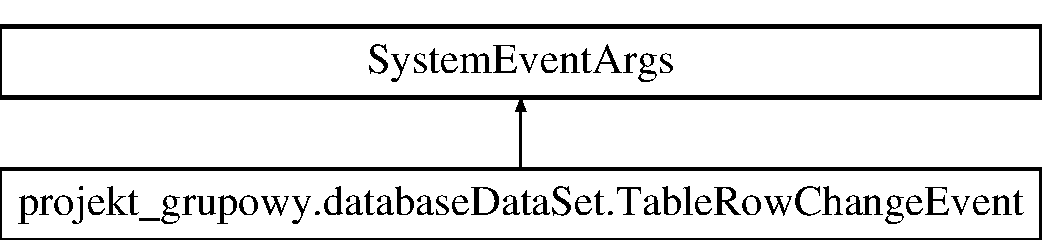
\includegraphics[height=2.000000cm]{classprojekt__grupowy_1_1database_data_set_1_1_table_row_change_event}
\end{center}
\end{figure}
\subsection*{Public Member Functions}
\begin{DoxyCompactItemize}
\item 
\mbox{\Hypertarget{classprojekt__grupowy_1_1database_data_set_1_1_table_row_change_event_aee93ee140809170f422c34832af17cb5}\label{classprojekt__grupowy_1_1database_data_set_1_1_table_row_change_event_aee93ee140809170f422c34832af17cb5}} 
{\bfseries Table\+Row\+Change\+Event} (\hyperlink{classprojekt__grupowy_1_1database_data_set_1_1_table_row}{Table\+Row} row, global\+::\+System.\+Data.\+Data\+Row\+Action action)
\end{DoxyCompactItemize}
\subsection*{Properties}
\begin{DoxyCompactItemize}
\item 
\mbox{\Hypertarget{classprojekt__grupowy_1_1database_data_set_1_1_table_row_change_event_a6dce7b7206150eeea08aa491b409de26}\label{classprojekt__grupowy_1_1database_data_set_1_1_table_row_change_event_a6dce7b7206150eeea08aa491b409de26}} 
\hyperlink{classprojekt__grupowy_1_1database_data_set_1_1_table_row}{Table\+Row} {\bfseries Row}\hspace{0.3cm}{\ttfamily  \mbox{[}get\mbox{]}}
\item 
\mbox{\Hypertarget{classprojekt__grupowy_1_1database_data_set_1_1_table_row_change_event_a0a349af0d99f4e443f4136e4d91e8d18}\label{classprojekt__grupowy_1_1database_data_set_1_1_table_row_change_event_a0a349af0d99f4e443f4136e4d91e8d18}} 
global\+::\+System.\+Data.\+Data\+Row\+Action {\bfseries Action}\hspace{0.3cm}{\ttfamily  \mbox{[}get\mbox{]}}
\end{DoxyCompactItemize}


\subsection{Detailed Description}
Row event argument class /summary$>$ 

The documentation for this class was generated from the following file\+:\begin{DoxyCompactItemize}
\item 
projekt\+\_\+grupowy/database\+Data\+Set.\+Designer.\+cs\end{DoxyCompactItemize}

\hypertarget{classprojekt__grupowy_1_1database_data_set1_1_1_table_row_change_event}{}\section{projekt\+\_\+grupowy.\+database\+Data\+Set1.\+Table\+Row\+Change\+Event Class Reference}
\label{classprojekt__grupowy_1_1database_data_set1_1_1_table_row_change_event}\index{projekt\+\_\+grupowy.\+database\+Data\+Set1.\+Table\+Row\+Change\+Event@{projekt\+\_\+grupowy.\+database\+Data\+Set1.\+Table\+Row\+Change\+Event}}


Row event argument class /summary$>$  


Inheritance diagram for projekt\+\_\+grupowy.\+database\+Data\+Set1.\+Table\+Row\+Change\+Event\+:\begin{figure}[H]
\begin{center}
\leavevmode
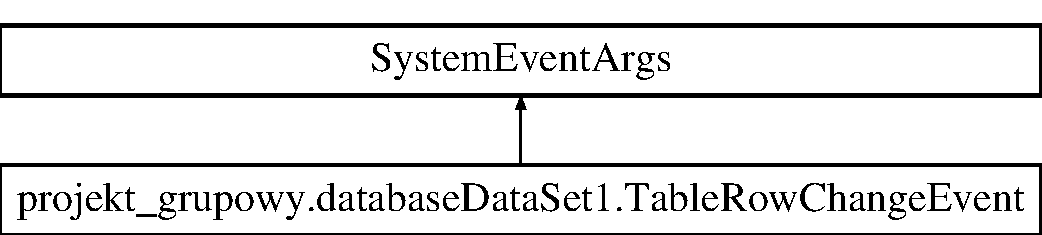
\includegraphics[height=2.000000cm]{classprojekt__grupowy_1_1database_data_set1_1_1_table_row_change_event}
\end{center}
\end{figure}
\subsection*{Public Member Functions}
\begin{DoxyCompactItemize}
\item 
\mbox{\Hypertarget{classprojekt__grupowy_1_1database_data_set1_1_1_table_row_change_event_a03c7dbcda15c031f6ad8d63ad94400fd}\label{classprojekt__grupowy_1_1database_data_set1_1_1_table_row_change_event_a03c7dbcda15c031f6ad8d63ad94400fd}} 
{\bfseries Table\+Row\+Change\+Event} (\hyperlink{classprojekt__grupowy_1_1database_data_set1_1_1_table_row}{Table\+Row} row, global\+::\+System.\+Data.\+Data\+Row\+Action action)
\end{DoxyCompactItemize}
\subsection*{Properties}
\begin{DoxyCompactItemize}
\item 
\mbox{\Hypertarget{classprojekt__grupowy_1_1database_data_set1_1_1_table_row_change_event_adc892b45f5d466eb863c982393c12488}\label{classprojekt__grupowy_1_1database_data_set1_1_1_table_row_change_event_adc892b45f5d466eb863c982393c12488}} 
\hyperlink{classprojekt__grupowy_1_1database_data_set1_1_1_table_row}{Table\+Row} {\bfseries Row}\hspace{0.3cm}{\ttfamily  \mbox{[}get\mbox{]}}
\item 
\mbox{\Hypertarget{classprojekt__grupowy_1_1database_data_set1_1_1_table_row_change_event_a3dde47339b69ab62914a0a85dee89834}\label{classprojekt__grupowy_1_1database_data_set1_1_1_table_row_change_event_a3dde47339b69ab62914a0a85dee89834}} 
global\+::\+System.\+Data.\+Data\+Row\+Action {\bfseries Action}\hspace{0.3cm}{\ttfamily  \mbox{[}get\mbox{]}}
\end{DoxyCompactItemize}


\subsection{Detailed Description}
Row event argument class /summary$>$ 

The documentation for this class was generated from the following file\+:\begin{DoxyCompactItemize}
\item 
projekt\+\_\+grupowy/database\+Data\+Set1.\+Designer.\+cs\end{DoxyCompactItemize}

\hypertarget{classprojekt__grupowy_1_1database_data_set_table_adapters_1_1_table_table_adapter}{}\section{projekt\+\_\+grupowy.\+database\+Data\+Set\+Table\+Adapters.\+Table\+Table\+Adapter Class Reference}
\label{classprojekt__grupowy_1_1database_data_set_table_adapters_1_1_table_table_adapter}\index{projekt\+\_\+grupowy.\+database\+Data\+Set\+Table\+Adapters.\+Table\+Table\+Adapter@{projekt\+\_\+grupowy.\+database\+Data\+Set\+Table\+Adapters.\+Table\+Table\+Adapter}}


Represents the connection and commands used to retrieve and save data. /summary$>$  


Inheritance diagram for projekt\+\_\+grupowy.\+database\+Data\+Set\+Table\+Adapters.\+Table\+Table\+Adapter\+:\begin{figure}[H]
\begin{center}
\leavevmode
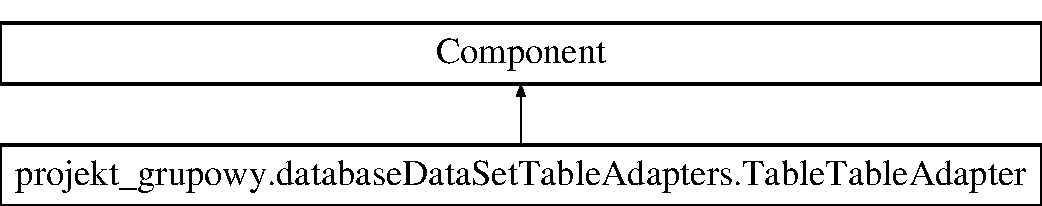
\includegraphics[height=2.000000cm]{classprojekt__grupowy_1_1database_data_set_table_adapters_1_1_table_table_adapter}
\end{center}
\end{figure}
\subsection*{Public Member Functions}
\begin{DoxyCompactItemize}
\item 
\mbox{\Hypertarget{classprojekt__grupowy_1_1database_data_set_table_adapters_1_1_table_table_adapter_ace766f9057ac5bd14bc51289934f7257}\label{classprojekt__grupowy_1_1database_data_set_table_adapters_1_1_table_table_adapter_ace766f9057ac5bd14bc51289934f7257}} 
virtual int {\bfseries Fill} (\hyperlink{classprojekt__grupowy_1_1database_data_set_1_1_table_data_table}{database\+Data\+Set.\+Table\+Data\+Table} data\+Table)
\item 
\mbox{\Hypertarget{classprojekt__grupowy_1_1database_data_set_table_adapters_1_1_table_table_adapter_addaae946c2860e16b770bd5ccd0bd95c}\label{classprojekt__grupowy_1_1database_data_set_table_adapters_1_1_table_table_adapter_addaae946c2860e16b770bd5ccd0bd95c}} 
virtual \hyperlink{classprojekt__grupowy_1_1database_data_set_1_1_table_data_table}{database\+Data\+Set.\+Table\+Data\+Table} {\bfseries Get\+Data} ()
\item 
\mbox{\Hypertarget{classprojekt__grupowy_1_1database_data_set_table_adapters_1_1_table_table_adapter_aa99c217f49e294ac250f80c25319bff5}\label{classprojekt__grupowy_1_1database_data_set_table_adapters_1_1_table_table_adapter_aa99c217f49e294ac250f80c25319bff5}} 
virtual int {\bfseries Search\+Surname} (\hyperlink{classprojekt__grupowy_1_1database_data_set_1_1_table_data_table}{database\+Data\+Set.\+Table\+Data\+Table} data\+Table, string Surname)
\item 
\mbox{\Hypertarget{classprojekt__grupowy_1_1database_data_set_table_adapters_1_1_table_table_adapter_a68ea68db5595a8527d78b01f4eba364c}\label{classprojekt__grupowy_1_1database_data_set_table_adapters_1_1_table_table_adapter_a68ea68db5595a8527d78b01f4eba364c}} 
virtual int {\bfseries Update} (\hyperlink{classprojekt__grupowy_1_1database_data_set_1_1_table_data_table}{database\+Data\+Set.\+Table\+Data\+Table} data\+Table)
\item 
\mbox{\Hypertarget{classprojekt__grupowy_1_1database_data_set_table_adapters_1_1_table_table_adapter_a86945efeb90b97afc51c0065cf7fc4c9}\label{classprojekt__grupowy_1_1database_data_set_table_adapters_1_1_table_table_adapter_a86945efeb90b97afc51c0065cf7fc4c9}} 
virtual int {\bfseries Update} (\hyperlink{classprojekt__grupowy_1_1database_data_set}{database\+Data\+Set} data\+Set)
\item 
\mbox{\Hypertarget{classprojekt__grupowy_1_1database_data_set_table_adapters_1_1_table_table_adapter_a0ba343619ac2126cb0030d37ebe48b07}\label{classprojekt__grupowy_1_1database_data_set_table_adapters_1_1_table_table_adapter_a0ba343619ac2126cb0030d37ebe48b07}} 
virtual int {\bfseries Update} (global\+::\+System.\+Data.\+Data\+Row data\+Row)
\item 
\mbox{\Hypertarget{classprojekt__grupowy_1_1database_data_set_table_adapters_1_1_table_table_adapter_a2b4a5f38949b32b8739c9b76baa5357b}\label{classprojekt__grupowy_1_1database_data_set_table_adapters_1_1_table_table_adapter_a2b4a5f38949b32b8739c9b76baa5357b}} 
virtual int {\bfseries Update} (global\+::\+System.\+Data.\+Data\+Row\mbox{[}$\,$\mbox{]} data\+Rows)
\item 
\mbox{\Hypertarget{classprojekt__grupowy_1_1database_data_set_table_adapters_1_1_table_table_adapter_ac64668e5af22effed944357e78c42d83}\label{classprojekt__grupowy_1_1database_data_set_table_adapters_1_1_table_table_adapter_ac64668e5af22effed944357e78c42d83}} 
virtual int {\bfseries Delete} (int Original\+\_\+\+Customer\+ID, string Original\+\_\+\+Name, string Original\+\_\+\+Surname, string Original\+\_\+\+Phone, string Original\+\_\+\+Brand, string Original\+\_\+\+Model)
\item 
\mbox{\Hypertarget{classprojekt__grupowy_1_1database_data_set_table_adapters_1_1_table_table_adapter_a4db11105cace274066c275f9118fae26}\label{classprojekt__grupowy_1_1database_data_set_table_adapters_1_1_table_table_adapter_a4db11105cace274066c275f9118fae26}} 
virtual int {\bfseries Insert} (int Customer\+ID, string Name, string Surname, string Phone, string Brand, string Model)
\item 
\mbox{\Hypertarget{classprojekt__grupowy_1_1database_data_set_table_adapters_1_1_table_table_adapter_a4981ba25dd25262541d005be45a18772}\label{classprojekt__grupowy_1_1database_data_set_table_adapters_1_1_table_table_adapter_a4981ba25dd25262541d005be45a18772}} 
virtual int {\bfseries Update} (int Customer\+ID, string Name, string Surname, string Phone, string Brand, string Model, int Original\+\_\+\+Customer\+ID, string Original\+\_\+\+Name, string Original\+\_\+\+Surname, string Original\+\_\+\+Phone, string Original\+\_\+\+Brand, string Original\+\_\+\+Model)
\item 
\mbox{\Hypertarget{classprojekt__grupowy_1_1database_data_set_table_adapters_1_1_table_table_adapter_a9f9377d4e6fec08065bed93c19395725}\label{classprojekt__grupowy_1_1database_data_set_table_adapters_1_1_table_table_adapter_a9f9377d4e6fec08065bed93c19395725}} 
virtual int {\bfseries Update} (string Name, string Surname, string Phone, string Brand, string Model, int Original\+\_\+\+Customer\+ID, string Original\+\_\+\+Name, string Original\+\_\+\+Surname, string Original\+\_\+\+Phone, string Original\+\_\+\+Brand, string Original\+\_\+\+Model)
\end{DoxyCompactItemize}
\subsection*{Properties}
\begin{DoxyCompactItemize}
\item 
\mbox{\Hypertarget{classprojekt__grupowy_1_1database_data_set_table_adapters_1_1_table_table_adapter_ad53e7649f9f3abef0b023deb1a49e262}\label{classprojekt__grupowy_1_1database_data_set_table_adapters_1_1_table_table_adapter_ad53e7649f9f3abef0b023deb1a49e262}} 
global\+::\+System.\+Data.\+Sql\+Client.\+Sql\+Command \mbox{[}$\,$\mbox{]} {\bfseries Command\+Collection}\hspace{0.3cm}{\ttfamily  \mbox{[}get\mbox{]}}
\item 
\mbox{\Hypertarget{classprojekt__grupowy_1_1database_data_set_table_adapters_1_1_table_table_adapter_a5b6398a078e60df017cb3a44f60dfdb9}\label{classprojekt__grupowy_1_1database_data_set_table_adapters_1_1_table_table_adapter_a5b6398a078e60df017cb3a44f60dfdb9}} 
bool {\bfseries Clear\+Before\+Fill}\hspace{0.3cm}{\ttfamily  \mbox{[}get, set\mbox{]}}
\end{DoxyCompactItemize}


\subsection{Detailed Description}
Represents the connection and commands used to retrieve and save data. /summary$>$ 

The documentation for this class was generated from the following file\+:\begin{DoxyCompactItemize}
\item 
projekt\+\_\+grupowy/database\+Data\+Set.\+Designer.\+cs\end{DoxyCompactItemize}

\hypertarget{classprojekt__grupowy_1_1database_data_set1_table_adapters_1_1_table_table_adapter}{}\section{projekt\+\_\+grupowy.\+database\+Data\+Set1\+Table\+Adapters.\+Table\+Table\+Adapter Class Reference}
\label{classprojekt__grupowy_1_1database_data_set1_table_adapters_1_1_table_table_adapter}\index{projekt\+\_\+grupowy.\+database\+Data\+Set1\+Table\+Adapters.\+Table\+Table\+Adapter@{projekt\+\_\+grupowy.\+database\+Data\+Set1\+Table\+Adapters.\+Table\+Table\+Adapter}}


Represents the connection and commands used to retrieve and save data. /summary$>$  


Inheritance diagram for projekt\+\_\+grupowy.\+database\+Data\+Set1\+Table\+Adapters.\+Table\+Table\+Adapter\+:\begin{figure}[H]
\begin{center}
\leavevmode
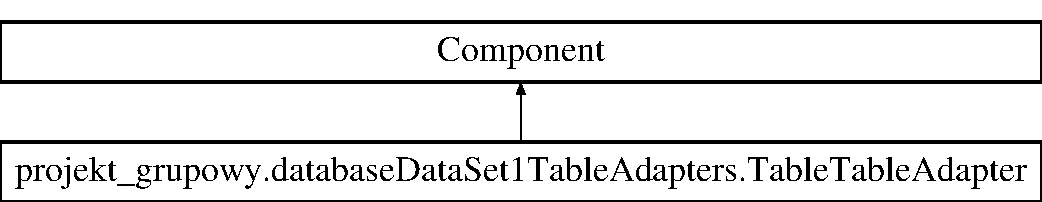
\includegraphics[height=2.000000cm]{classprojekt__grupowy_1_1database_data_set1_table_adapters_1_1_table_table_adapter}
\end{center}
\end{figure}
\subsection*{Public Member Functions}
\begin{DoxyCompactItemize}
\item 
\mbox{\Hypertarget{classprojekt__grupowy_1_1database_data_set1_table_adapters_1_1_table_table_adapter_ac51d79a2e0b77798ce38b010948f613c}\label{classprojekt__grupowy_1_1database_data_set1_table_adapters_1_1_table_table_adapter_ac51d79a2e0b77798ce38b010948f613c}} 
virtual int {\bfseries Fill} (\hyperlink{classprojekt__grupowy_1_1database_data_set1_1_1_table_data_table}{database\+Data\+Set1.\+Table\+Data\+Table} data\+Table)
\item 
\mbox{\Hypertarget{classprojekt__grupowy_1_1database_data_set1_table_adapters_1_1_table_table_adapter_ae0d15147aa5ec8d10faf60389f8dfeb3}\label{classprojekt__grupowy_1_1database_data_set1_table_adapters_1_1_table_table_adapter_ae0d15147aa5ec8d10faf60389f8dfeb3}} 
virtual \hyperlink{classprojekt__grupowy_1_1database_data_set1_1_1_table_data_table}{database\+Data\+Set1.\+Table\+Data\+Table} {\bfseries Get\+Data} ()
\item 
\mbox{\Hypertarget{classprojekt__grupowy_1_1database_data_set1_table_adapters_1_1_table_table_adapter_a8da9816e4ab07c692004e9b6ee4bbfa8}\label{classprojekt__grupowy_1_1database_data_set1_table_adapters_1_1_table_table_adapter_a8da9816e4ab07c692004e9b6ee4bbfa8}} 
virtual int {\bfseries Update} (\hyperlink{classprojekt__grupowy_1_1database_data_set1_1_1_table_data_table}{database\+Data\+Set1.\+Table\+Data\+Table} data\+Table)
\item 
\mbox{\Hypertarget{classprojekt__grupowy_1_1database_data_set1_table_adapters_1_1_table_table_adapter_a6d48193f816337b62976432af96191f1}\label{classprojekt__grupowy_1_1database_data_set1_table_adapters_1_1_table_table_adapter_a6d48193f816337b62976432af96191f1}} 
virtual int {\bfseries Update} (\hyperlink{classprojekt__grupowy_1_1database_data_set1}{database\+Data\+Set1} data\+Set)
\item 
\mbox{\Hypertarget{classprojekt__grupowy_1_1database_data_set1_table_adapters_1_1_table_table_adapter_af161b57d120e3462d8ae0266df9c67f5}\label{classprojekt__grupowy_1_1database_data_set1_table_adapters_1_1_table_table_adapter_af161b57d120e3462d8ae0266df9c67f5}} 
virtual int {\bfseries Update} (global\+::\+System.\+Data.\+Data\+Row data\+Row)
\item 
\mbox{\Hypertarget{classprojekt__grupowy_1_1database_data_set1_table_adapters_1_1_table_table_adapter_aeac8d61ed8d1324df244262302037782}\label{classprojekt__grupowy_1_1database_data_set1_table_adapters_1_1_table_table_adapter_aeac8d61ed8d1324df244262302037782}} 
virtual int {\bfseries Update} (global\+::\+System.\+Data.\+Data\+Row\mbox{[}$\,$\mbox{]} data\+Rows)
\item 
\mbox{\Hypertarget{classprojekt__grupowy_1_1database_data_set1_table_adapters_1_1_table_table_adapter_a899333eb1375b0f5a55b66d24def491e}\label{classprojekt__grupowy_1_1database_data_set1_table_adapters_1_1_table_table_adapter_a899333eb1375b0f5a55b66d24def491e}} 
virtual int {\bfseries Delete} (int Original\+\_\+\+Customer\+ID, string Original\+\_\+\+Name, string Original\+\_\+\+Surname, string Original\+\_\+\+Phone, string Original\+\_\+\+Brand, string Original\+\_\+\+Model)
\item 
\mbox{\Hypertarget{classprojekt__grupowy_1_1database_data_set1_table_adapters_1_1_table_table_adapter_a1237de20ecf9571ab5b63074a94d61a4}\label{classprojekt__grupowy_1_1database_data_set1_table_adapters_1_1_table_table_adapter_a1237de20ecf9571ab5b63074a94d61a4}} 
virtual int {\bfseries Insert} (int Customer\+ID, string Name, string Surname, string Phone, string Brand, string Model)
\item 
\mbox{\Hypertarget{classprojekt__grupowy_1_1database_data_set1_table_adapters_1_1_table_table_adapter_aa2fe5234ce8dd95214a82117bbd7cadc}\label{classprojekt__grupowy_1_1database_data_set1_table_adapters_1_1_table_table_adapter_aa2fe5234ce8dd95214a82117bbd7cadc}} 
virtual int {\bfseries Update} (int Customer\+ID, string Name, string Surname, string Phone, string Brand, string Model, int Original\+\_\+\+Customer\+ID, string Original\+\_\+\+Name, string Original\+\_\+\+Surname, string Original\+\_\+\+Phone, string Original\+\_\+\+Brand, string Original\+\_\+\+Model)
\item 
\mbox{\Hypertarget{classprojekt__grupowy_1_1database_data_set1_table_adapters_1_1_table_table_adapter_a1267627bd5da469bda400434a2e1af5e}\label{classprojekt__grupowy_1_1database_data_set1_table_adapters_1_1_table_table_adapter_a1267627bd5da469bda400434a2e1af5e}} 
virtual int {\bfseries Update} (string Name, string Surname, string Phone, string Brand, string Model, int Original\+\_\+\+Customer\+ID, string Original\+\_\+\+Name, string Original\+\_\+\+Surname, string Original\+\_\+\+Phone, string Original\+\_\+\+Brand, string Original\+\_\+\+Model)
\end{DoxyCompactItemize}
\subsection*{Properties}
\begin{DoxyCompactItemize}
\item 
\mbox{\Hypertarget{classprojekt__grupowy_1_1database_data_set1_table_adapters_1_1_table_table_adapter_acd520dcfc12f0d3694af44091909dd81}\label{classprojekt__grupowy_1_1database_data_set1_table_adapters_1_1_table_table_adapter_acd520dcfc12f0d3694af44091909dd81}} 
global\+::\+System.\+Data.\+Sql\+Client.\+Sql\+Command \mbox{[}$\,$\mbox{]} {\bfseries Command\+Collection}\hspace{0.3cm}{\ttfamily  \mbox{[}get\mbox{]}}
\item 
\mbox{\Hypertarget{classprojekt__grupowy_1_1database_data_set1_table_adapters_1_1_table_table_adapter_a53fd5eb3db03d603480e63f5bd36e846}\label{classprojekt__grupowy_1_1database_data_set1_table_adapters_1_1_table_table_adapter_a53fd5eb3db03d603480e63f5bd36e846}} 
bool {\bfseries Clear\+Before\+Fill}\hspace{0.3cm}{\ttfamily  \mbox{[}get, set\mbox{]}}
\end{DoxyCompactItemize}


\subsection{Detailed Description}
Represents the connection and commands used to retrieve and save data. /summary$>$ 

The documentation for this class was generated from the following file\+:\begin{DoxyCompactItemize}
\item 
projekt\+\_\+grupowy/database\+Data\+Set1.\+Designer.\+cs\end{DoxyCompactItemize}

%--- End generated contents ---

% Index
\backmatter
\newpage
\phantomsection
\clearemptydoublepage
\addcontentsline{toc}{chapter}{Index}
\printindex

\end{document}
